\documentclass[titlepage,12pt,a4paper]{article}
%\documentclass[12pt]{report} 
%\usepackage[y4project]{edmaths} 
\usepackage[utf8x]{inputenc}
\usepackage[T1]{fontenc}
\usepackage{mathptmx} % Use Times Font
%\usepackage{listings}
\usepackage{amsmath}
\usepackage{mathtools}
\usepackage{amssymb}
\usepackage{tikz-cd}

\usepackage{enumerate}
%\usepackage{mathtools}
%\usepackage{theoremref}
\usepackage{amsthm}
\newcounter{thm}
\numberwithin{thm}{section}

\theoremstyle{plain}
\newtheorem{theorem}{Theorem}[thm]
\newtheorem{corollary}{Corollary}[thm]
\newtheorem{lemma}[thm]{Lemma}
\newtheorem{prop}[thm]{Proposition}
\newtheorem{proposition}[thm]{Proposition}

\theoremstyle{definition}
\newtheorem{definition}[thm]{Definition}
%\theoremstyle{remark}
\newtheorem{remark}[thm]{Remark}
\newtheorem{example}[thm]{Example}
\bibliographystyle{apalike}
\newcommand{\dsum}{\oplus}
\newcommand{\iso}{\cong}
\newcommand{\homeo}{\cong}
\newcommand{\homotopic}{\simeq}
\newcommand{\defn}[1]{\textbf{#1}}
\newcommand{\cat}[1]{\mathcal{#1}}
\newcommand{\RP}[1]{\mathbb{RP}^{#1}}
\newcommand{\CP}[1]{\mathbb{CP}^{#1}}
\newcommand{\HP}[1]{\mathbb{HP}^{#1}}
\newcommand{\Top}[1]{\mathbf{Top}_{#1}}
\newcommand{\Mod}[1]{\ (\mathrm{mod}\ #1)}
\newcommand{\C}{\mathbf{C}}
\newcommand*\bigcdot{\mathpalette\bigcdot@{.5}}

\title{Axiomatic Homology Theory}
\author{Malthe Sporring\\ Supervised by Clark Barwick}
\date{\today}


\begin{document}
\maketitle


\tableofcontents
\newpage
\section{Notes and acknowledgements}
This text provides an introduction to homology theory from an axiomatic point of view. The reader is assumed to have knowledge of undergraduate level Algebra and Algebraic Topology, particularly \textit{groups, homotopies, homotopy equivalences} and \textit{quotient spaces}.

I am very grateful to Clark Barwick for supervising this project and for sharing both his knowledge and passion for the subject. I also wish to extend my gratitude to the University of Edinburgh School of Mathematics Vacation Scholarship and College Vacation Scholarship funds for funding this project.
\newpage
\section{Introduction}
One of the goals of algebraic topology is classifying spaces up to some definition of equivalence, typically homotopy equivalence. Establishing equivalence can be tedious, as it often requires the construction of an explicit homotopy equivalence. However, \textit{inequivalence} is often easier to establish by calculating \defn{homotopy invariants}. These are properties of a space that are preserved by homotopy equivalences, hence if two spaces have different invariants, they cannot be homotopy equivalent. One of the first major homotopy invariances the undergraduate student encounters are the homotopy groups $\pi_n(X),n\in \mathbb{N}\cup \{0\}$: the groups of maps $f:S^{n}\rightarrow X$ with some base point. The homotopy groups carry a lot of geometric information, but are notoriously difficult to compute. Even for a simple space like the $2$-sphere $S^2$, it is not obvious that there are non-trivial maps $S^3\rightarrow S^2$ (we show that such a map exists in section \ref{sec-complex-projective-space}), and it is even less obvious what the higher homotopy groups are. The groups $\pi_n(S^2)$ do not seem to follow a pattern, and remain an active area of research. Only recently in 2015 was it proven that $\pi_n(S^2)$ is not zero for all $n\geq 2$ \cite{Ivanov}.

To avoid these complications, we would like to find homotopy invariances that are easier to compute, and ideally, not at the cost of too much geometric information. The homology groups $H_n(X)$ are an example of such a homotopy invariant. Like the homotopy groups, they are a sequence of groups, one for each $n\in \mathbb{Z}$, but they are much simpler and easier to compute. For example, the spheres have the simple structure $$H_n(S^m)=\begin{cases}\mathbb{Z} & n=0,m\\ 0 & \text{otherwise}\end{cases}$$
Part of the reason why they are easier to compute is that they come with extra structure, most importantly a \defn{long exact sequence}, which, broadly speaking, relates the homology groups $H_nX$ to each other and to the homology groups $H_nA$ of a subspace $A\subseteq X$. Therefore, the more you know about some of the homology groups of a space and a subspace, the easier it is to calculate the rest.

Historically, homology groups were produced from a number of geometric methods. It was Eilenberg and Steenrod who united the different homology theories by laying out a set of axioms that all homology theories satisfy \ref{Eilenberg}. In this text, we will take such an axiomatic approach, proving all results directly from the axioms. In some ways this approach more directly shows the point of homology theory. As will become clear, we will very rarely want for the geometric construction, and in fact all (ordinary) homology theories which satisfy the same Eilenberg-Steenrod axioms and initial conditions are equivalent; the geometric construction contributes no more than can be captured in the axioms (REFERENCE). It is therefore believable that the main role of a geometric construction of homology theory is to prove the Eilenberg-Steenrod Axioms for that theory. For the results to be true we have to take given that there exists at least one homology theory which satisfies the axioms. Proving this is a major undertaking worth its own project. Singular Homology is an example of a homology theory which satisfies our assumptions, and the reader is invited to confirm that it satisfies the axioms in \cite{Hatcher}.

Homology theory is best understood in the language of category theory and chain complexes, which sections \ref{sec-category-theory} and \ref{sec-chain-complexes} are devoted to. In section \ref{sec-axioms}, we lay out the Eilenberg-Steenrod axioms and prove some immediate results for a general ordinary homology theory, most importantly the homology groups of the $n$-sphere. In the following sections we make the choice $H_0 \cdot=\mathbb{Z}$, which corresponds to Singular Homology. In sections \ref{sec-Mayer-Vietoris}, \ref{sec-degree-maps} and \ref{sec-cellular-homology} we lay out three practical methods for calculating homology groups; The Mayer-Vietoris Sequence, degree maps and Cellular Homology, and use them to prove some fascinating results.
\section{Category theory}\label{sec-category-theory}
The language of category theory was invented specifically for homology theory but has since then become an entire field of itself with many applications \cite{Marquis}. It is a very general construction, as many familiar constructions form categories, including groups, rings, vector spaces and topological spaces. Informally, a category is a collection of "objects" and "maps between them". In above-mentioned cases, the objects are sets with some structure, and the maps are functions that satisfy some structure-preserving property. However, the definition of a category is more general than this, and there are categories whose objects look nothing like sets and whose maps look nothing like functions between sets.

\begin{definition}
A category $\cat{A}$ is
\begin{itemize}
    \item a \defn{collection}\footnote{The term \defn{collection} is similar to a set, with some technical distinguishing properties laid out in \cite{Leinster}.} of objects $ob(\cat{A})$,
    \item for each $A,B\in ob(\cat{A})$ a collection $\cat{A}(A,B)$ of maps from $A$ to $B$,
    \item a composition function $\circ:\cat{A}(A,B)\times \cat{A}(B,C)\rightarrow \cat{A}(A,C)$,
\end{itemize}
which satisfy the following properties:

\begin{enumerate}[(a)]
\item \textbf{Associativity}: $(f\circ g)\circ h=f\circ(g\circ f)$,
\item \textbf{Identity laws}: For each $A\in ob(\cat{A})$ there is a unique map $id_A\in \cat{A}(A,A)$ with the property that $id_A\circ f$=$f$ and $g\circ id_A=g$ for every $f\in \cat{A}(B,A)$ and $g\in \cat{A}(A,B)$.
\end{enumerate}
\end{definition}
We often write $A\in \cat{A}$ to mean $A\in ob(\cat{A})$, and $fg$ to mean $f\circ g$.
\par Categories are best understood through examples, of which we give a few. Many more examples are given in \cite{Leinster}.

\begin{example}
The following are categories.
\begin{enumerate}[(a)]

\item The empty category $\emptyset$ with no objects and no maps.
\item A one-object category $\{A\}$ with only the identity map $id_A$.

\item $\mathbf{Top}$ is a category, where spaces are topological spaces, and the maps are all continuous maps. This is because the identity map is always continuous, and compositions of continuous maps are continuous.

\item We have similar constructions for other "sets with structure" and "structure-preserving maps" such as $\mathbf{Vec}$ the category of vector spaces and linear maps, and $\mathbf{Grp}$, the category of groups and homomorphisms.
\item Many categories can be found as subcategories of previous examples. For example, we have the subcategory $\mathbf{Ab}\subset \mathbf{Grp}$ of abelian groups and homomorphisms between them.
\item Finally, here is an example of a category that cannot be interpreted as "sets" and "structure-preserving maps": 
% https://tikzcd.yichuanshen.de/#N4Igdg9gJgpgziAXAbVABwnAlgFyxMJZABgBpiBdUkANwEMAbAVxiRAEEQBfU9TXfIRQAmclVqMWbAELdxMKAHN4RUADMAThAC2SMiBwQ91BhAhoiZNYzgxxDOgCMYDAAr88BNhqyKAFjgg1PTMrIggWFAA+pw86lq6iACM1IZIKSCm5pak1gy29k4u7tieQiA+-oHBkmER0bJxIJo6xgZGyTWhbGpBIM5gUEgAzMRNLYkZaYj6A0OIo11S4YrcvM0JbdP6WRYoSQAcVjZ2JkVuHoLevgF9Icsgir1cFFxAA
\[\begin{tikzcd}
A \arrow["id_A"', loop, distance=2em, in=305, out=235] \arrow[rr, "f", bend left] \arrow["gf"', loop, distance=2em, in=125, out=55] &  & B \arrow["id_B"', loop, distance=2em, in=305, out=235] \arrow[ll, "g", bend left]
\end{tikzcd}\]
If we tried to interpret this as two one-element sets $A$ and $B$ together with the only maps $f,g$ between them, we run into trouble, as there are two distinct maps from $A$ to itself! However this category satisfies the definitions: we have identities, and for every two maps we have defined their compositions
$$fg=id_B, f(gf)=f,(gf)g=g,(gf)(gf)=gf$$
These compositions are forced upon us by the associativity requirement, for example $f(gf)=(fg)f=(id_A)f=f$, and $(gf)(gf)=g(fg)f=gf$. One might think $gf$ contradicts the uniqueness of the identity requirement, but it does not, as $(gf)id_A=gf\neq id_A$. 

\end{enumerate}\end{example}
\par Two definitions that will play a big role in our study are the notions of "maps between categories" and "maps between maps between categories". These are called \defn{functors} and \defn{natural transformations}, respectively.

\begin{definition}
A \defn{functor} $F:\cat{C}\rightarrow\cat{H}$ between two categories is a function assigning each $X\in ob(\cat{C})$ to some $F(X)\in ob(\cat{H})$, and each $f\in \cat{C}(A,B)$ to some $F(f)\in \cat{H}(F(A),F(B))$, such that
\begin{enumerate}[(a)]
\item $F(f\circ g)=F(f)\circ F(g)$
\item $F(id_A)=id_{F(A)}$
\end{enumerate}
\end{definition}
The definition of a functor is set up such that it takes commutative diagrams to commutative diagrams. I.e. if this commutative diagram is in $\cat{C}$,
% https://tikzcd.yichuanshen.de/#N4Igdg9gJgpgziAXAbVABwnAlgFyxMJZABgBpiBdUkANwEMAbAVxiRAEEQBfU9TXfIRQBGclVqMWbAELdeIDNjwEio4ePrNWiEAGE5fJYKJl11TVJ0ARbuJhQA5vCKgAZgCcIAWyRkQOCCRRCS02VwMQD28g6gCkACZzSW0QBwion0Q-OMQAZiTQnQArEGoGOgAjGAYABX5lIRAGGFccdM9M-P9AxESQyxAAC1suIA
\[\begin{tikzcd}
A \arrow[r, "f"] \arrow[d, "j"] & B \arrow[d, "g"] \\
D \arrow[r, "h"]                & C               
\end{tikzcd}\]
then the following commutative diagram is in $\cat{H}$:
% https://tikzcd.yichuanshen.de/#N4Igdg9gJgpgziAXAbVABwnAlgFyxMJZABgBpiBdUkANwEMAbAVxiRADEAKAQQEoQAvqXSZc+QigCM5KrUYs2XAEL8hI7HgJFpk2fWatEHTgGFVwkBg3iiZXdX0KjXACKrZMKAHN4RUADMAJwgAWyQyEBwIJGk5A0VOf3MA4LDEWKikACYHeUNjL2SQINDw6kzEAGZc+OdOACt+agY6ACMYBgAFUU0JEAYYfxxBCxK06sjoxBy4p2MAC3cBIA
\[\begin{tikzcd}
F(A) \arrow[r, "F(f)"] \arrow[d, "F(j)"] & F(B) \arrow[d, "F(g)"] \\
F(D) \arrow[r, "F(h)"]                   & F(C)                  
\end{tikzcd}\]

\begin{example}
There is a functor $F:\mathbf{Grp}\rightarrow \mathbf{Set}$ which forgets the group structure. Explicitly, it maps each group $G\in \mathbf{Grp}$ to the underlying set in $\mathbf{Set}$, and each homomorphism $f$ to the underlying function between sets. This functor is appropriately named the \defn{forgetful functor}.
\end{example}

\begin{example}
There is a functor $\mathbf{Top}:\mathbf{Grp}$ which takes each topological space $X$ to its fundamental group $\pi_1(X)$.\footnote{Technically, the domain should be the category of \defn{based Topological spaces} $\mathbf{Top_{\bullet}}$, whose objects are spaces with a point, and whose maps are base-point preserving maps.} This is well-defined since continuous maps $f$ give rise to homomorphisms $f^*$ between fundamental groups, the identity map gives rise to the identity homomorphism, and $(fg)^*=f^*g^*$.
\end{example}

\begin{definition}
A \defn{natural transformation} $\alpha:F\rightarrow G$ between functors $F,G:\cat{A}\rightarrow \cat{B}$ is a family of functions $(\alpha_A:F(A)\rightarrow G(A))_{A\in \cat{A}}$ between objects in $\cat{B}$ such that any map $f:A\rightarrow B$ in $\cat{A}$ gives rise to a commutative diagram

% https://tikzcd.yichuanshen.de/#N4Igdg9gJgpgziAXAbVABwnAlgFyxMJZABgBpiBdUkANwEMAbAVxiRADEAKAQQEoQAvqXSZc+QijIBGKrUYs2XAEL8hI7HgJEppGdXrNWiDpxWDhIDBvHbysgwuMBxHqtkwoAc3hFQAMwAnCABbJDIQHAgkAGZ9eSMQAB1ExjQACzoAfW5zfyDQxB0IqMQAJjjDNmTUjMylXJBAkLDqSKQihwSuP1ULJoLY4qRyuUrnTh7BCgEgA
\[\begin{tikzcd}
F(A) \arrow[r, "\alpha_A"] \arrow[d, "F(f)"] & G(A) \arrow[d, "G(f)"] \\
F(B) \arrow[r, "\alpha_B"]                   & F(B)                  
\end{tikzcd}\]
\end{definition}
Functors and natural transformations are explored in-depth in \cite{Leinster}. For now, we will make do with the definitions. The properties we will use the most are that \textit{functors preserve commutative diagrams} and that \textit{natural transformations commute with functors} in the way specified by the above diagram. 
\section{Chain Complexes}\label{sec-chain-complexes}
\begin{definition}
A \defn{chain complex} is a family $(A_i)_{i\in\mathbb{Z}}$ of abelian groups, as well as a family $(f_i:A_i\rightarrow A_{i+1})_{i\in \mathbb{Z}}$ of homomorphisms between consecutive groups, such that $im(f_i)\subset ker(f_{i+1})$. If we have equality instead of inclusion, the family is called an \defn{exact sequence}.
\end{definition}

We distinguish between \defn{short} and \defn{long exact sequences}, where short exact sequences are sequences with three or fewer consecutive non-zero groups, i.e. sequences of the form

% https://tikzcd.yichuanshen.de/#N4Igdg9gJgpgziAXAbVABwnAlgFyxMJZABgBpiBdUkANwEMAbAVxiRGJAF9T1Nd9CKAIzkqtRizYBBLjxAZseAkQBMo6vWatEIAEKzeigUQDM68VrYBhA-L5LByACznNknR05iYUAObwiUAAzACcIAFskMhAcCCQRC3d2W1CI+OpYpDVE7RAglLDIxGzMxDMctl8CtLKMuMQXCo8uCk4gA
\[\begin{tikzcd}
0 \arrow[r, "0"] & A \arrow[r, "f"] & B \arrow[r, "g"] & C \arrow[r, "0"] & 0
\end{tikzcd}\]
All other exact sequences are called long exact sequences. 

\begin{example}
For any abelian group $A$ the following is a long exact sequence:
% https://tikzcd.yichuanshen.de/#N4Igdg9gJgpgziAXAbVABwnAlgFyxMJZARgBoAGAXVJADcBDAGwFcYkQBBEAX1PU1z5CKAEwVqdJq3Zde-bHgJEAzOJoMWbRJx58QGBUKIAWNZM3sAOpagQcCOfoGLhycmY3Tt12-Z4SYKABzeCJQADMAJwgAWyR3EBwIJDJzLxAsKF0I6LjEVKSkMTStEHJskCjYoppCxFUS9kyKqrzTROTEBM9S8u5KbiA
\[\begin{tikzcd}
\dots \arrow[r, "0"] & A \arrow[r, "id"] & A \arrow[r, "0"] & A \arrow[r, "id"] & \dots
\end{tikzcd}\]
\end{example}

\begin{remark}
The requirement that $im(f_i)\subseteq ker(f_{i+1})$  is equivalent to the requirement that $f_{i+1}\circ f_i=0$. This is clear from the definition: if $im(f_i)\subseteq ker(f_{i+1})$ then $$\forall x\in A_i, f_{i+1}\circ f_i (x)\in f_{i+1}(im(f_i))=\{0\}.$$ Additionally, if $\forall x\in A_i, f_{i+1}\circ f_i=0$ then $f_{i+1}(im(f_i))=\{0\}$.
\end{remark}


\begin{example}
Suppose the following is part of a long exact sequence of groups.
% https://tikzcd.yichuanshen.de/#N4Igdg9gJgpgziAXAbVABwnAlgFyxMJZARgBoAGAXVJADcBDAGwFcYkQBBEAX1PU1z5CKAEwVqdJq3YAhHnxAZseAkQDM4mgxZtEIAMLz+yoUQAsmyTvYARI4oErhyAKyXt0vQB0vUCDgReY0FVFHJ3KV0QHz8AngkYKABzeCJQADMAJwgAWyRwkBwIJDIrTxByeyzckpoipDEyqPSq7LzERvrEDSb2SqCQavaerrMBoaQ3QuLEcm5KbiA
\[\begin{tikzcd}
\dots \arrow[r] & A \arrow[r, "0"] & B \arrow[r, "f"] & C \arrow[r, "0"] & D \arrow[r] & \dots
\end{tikzcd}\]
We say this \defn{gives rise to} the following short exact sequence, as they carry the same information.
% https://tikzcd.yichuanshen.de/#N4Igdg9gJgpgziAXAbVABwnAlgFyxMJZABgBpiBdUkANwEMAbAVxiRGJAF9T1Nd9CKAIzkqtRizYAhLjxAZseAkQBMo6vWatEIAMKzeigUQDM68VrYdOYmFADm8IqABmAJwgBbJCJA4ISGoWkjouBiDuXkhkfgGIQtyuHt6IQf5IJjacQA
\[\begin{tikzcd}
0 \arrow[r] & B \arrow[r, "f"] & C \arrow[r] & 0
\end{tikzcd}\]
Note we can omit specifying any homomorphisms from or into $0$, as there is only one: the $0$-homomorphism. Since $0=im(0)=ker(f)$, $f$ is injective. Since $im(f)=ker(0)=C$, $f$ is surjective. Therefore $f$ is an isomorphism.
\end{example}

\begin{definition}
If there exist maps $f:A\rightarrow B$ and $g:B\rightarrow A$ between abelian groups such that $g\circ f = id_A$ then $g$ is called a \defn{retraction} of $f$. If alternatively $f\circ g=id_B$, then $f$ is called a \defn{section} of $f$.
\end{definition}
This definition formalises the idea of a "one-sided inverse".

\begin{prop}\label{short-seq-direct-sum}
Let the following be a short exact sequence
% https://tikzcd.yichuanshen.de/#N4Igdg9gJgpgziAXAbVABwnAlgFyxMJZABgBpiBdUkANwEMAbAVxiRGJAF9T1Nd9CKACzkqtRizYduvbHgJEAjKOr1mrRCACCXHiAxyBRAEwrx6tgCFds-gpQBmM2smaAwlzEwoAc3hFQADMAJwgAWyQyEBwIJGMZEBDwpBFo2MRFBKSIxFM0pCdzV0SbRNCcwpiU1QkNEB9PTiA
\[\begin{tikzcd}
0 \arrow[r] & A \arrow[r, "f"] & B \arrow[r, "g"] & C \arrow[r] & 0
\end{tikzcd}\]
\begin{enumerate}[(a)]
    \item If there exists a \defn{section} $s:C\rightarrow B$ of $g$, then $f$ and $s$ define an isomorphism $$(f+s):A\dsum C\rightarrow B$$
$$(a,c)\mapsto f(a)+s(c).$$
\item If there exists a \defn{retraction} $r:B\rightarrow A$ of $f$, then $r$ and $g$ define an isomorphism $$(r,g):B\rightarrow A\dsum C$$
$$b\mapsto (r(b),g(b)).$$
\end{enumerate}
\end{prop}

\begin{proof}
\begin{enumerate}[(a)]
\item First we show that $(f+s)$ is injective. By exactness we have that $f$ is injective, as $0=im(0)=ker(f)$, and that $g$ is surjective, as $im(g)=ker(0)=C$. Suppose $f(a)+s(c)=0$. Then $$0=g(0)=g(f(a)+s(c))=gf(a)+gs(c)=c$$
Which implies $c=0$. But then $0=f(a)$, which implies $a=0$ as $f$ is injective. Therefore $ker(f+s)=0$, so $(f+s)$ is injective.

Next we show $(f+s)$ is surjective. Let $b\in B$, $c=g(b)\in C$ and $a\in A$ be the unique element that maps to $b-sg(b)\in B$. This element exists, since $$g(b-s(g(b)))=g(b)-g(b)=0,$$ so $b-sg(b)\in ker(g)=im(f)$. It is unique by the injectivity of $f$. It follows that $$f(a)+s(c)=b-sg(b)+sg(b)=b,$$ so $(f,s)$ is surjective. It is therefore an isomorphism.

\item First we show that $(r,g)$ is injective. Suppose $(r(b),g(b))=(0,0)$. Then $g(b)=0,$ so $b\in ker(g)=im(f)$. Now $r$ is injective on $im(f)$, since $rf=id_A$. Therefore $r(b)=0\implies b=0$. So $(r,g)$ is injective.

Next we show $(r,g)$ is surjective. Let $(a,c)\in A\dsum C$. Since $g$ is surjective, there exists $b\in B$ such that $c=g(b)$. Let $x=f(a)+b-fr(b)\in B$. Then $g(x)=g(b)$, as $gf(-)=0$ by exactness. Additionally, $$r(x)=rf(a)+r(b)-rfr(b)=a+r(b)-r(b)=a,$$
since $rf=id_A$. It follows that $(r,g)$ is also surjective, so it is an isomorphism.
\end{enumerate}

\end{proof}

The next proposition is not necessarily about chain complexes, but is very much in the flavour of Proposition \ref{short-seq-direct-sum} and will be very useful in our study.

\begin{proposition}\label{retraction-iso}
If $f:A\rightarrow B$ admits a retraction $g:B\rightarrow A$, then $$B\iso im(f)\dsum ker(g)$$
\end{proposition}

\begin{proof}
We define a homomorphism $$h:B\rightarrow im(f)\dsum ker(g)$$
$$b\mapsto (fg(b),b-fg(b))$$
This is well defined as $fg(b)\in im(f)$ trivially, and $g(b-fg(b))=g(b)-g(b)=0$.
First we show $h$ is injective. Let $(fg(b),b-fg(b))=(0,0)$. Then $b-fg(b)=b=0$, as $fg(b)=0$, so $h$ is injective. Next we show $h$ is surjective. Let $(x,y)\in im(f)\dsum ker(g)$, and $a\in A$ be such that $f(a)=x$. Then $$h(x+y)=(fgf(a)+fg(y),f(a)+y-fgf(a))=(f(a),y)=(x,y),$$
as $gf=id_A$ and $g(y)=0$.
It follows that $h$ is surjective, so it is in fact an isomorphism.\end{proof}

We finish this section with a technical lemma that will become useful in section \ref{sec-axioms}.

\begin{lemma}[Braid lemma]\label{braid-lemma}
Suppose three long exact sequences and a chain complex make the following commutative diagram.

% https://tikzcd.yichuanshen.de/#N4Igdg9gJgpgziAXAbVABwnAlgFyxMJZARgBpiBdUkANwEMAbAVxiRAEEQBfU9TXfIRRkAzFVqMWbAELdeIDNjwEiAVnLj6zVohABxOXyWC1pMdS1TdACUML+yocgBMpZ5sk6QAYTuKBKigiGhaebAAifg4mQWYe2mwAolHGgcgALG7xViAAYikBTgBsWaEJugCSBY5EAAyktdle1THI9e5lOQDyLWn16U1svcUNg7rDRCUDnc1c4jBQAObwRKAAZgBOEAC2SPUgOBBImRLlIGsA+sR2mzvH1IdIJac5l843W7uIz4+IwSAAIxgYCgSAAtOkAJwzNiXEQfO6IMgHI6IE6WLwACyuCK+J1+6heWIu7x460+SEJv1cgOBoLR0KJbGx8LJ5wpiH2BOoQJBx0ZGLYixxbNuX2Rv2evPpEIFYV0ACsRfIxU8HqiAOwwxUk3FILUopA0wU61kqjlUzXakDC0nmxEG37-E02i5m8mI-6-AAc1su6T1iBpPut2IDoo5jN++2lSBEtQjiOIXNR+xdwtqgeT6qQyJdSszifFEtRyNjiDB8aLRpzSJp5fj1qV4ftXy9pf+5craflrvDFC4QA
\begin{tikzcd}
{} \arrow[rd, bend left]              &                                                      &                                       &                                                      &                                       &                                                   & {} \\
                                      & A \arrow[rd, "f_1"] \arrow[rr, "g_1", bend left=49]  &                                       & D \arrow[rr, "h_3", bend left=49] \arrow[rd, "g_2"]  &                                       & G \arrow[rd, "h_4"] \arrow[ru, "j_4", bend left]  &    \\
O \arrow[ru, "g_0"] \arrow[rd, "j_0"] &                                                      & C \arrow[rd, "f_2"] \arrow[ru, "h_2"] &                                                      & F \arrow[ru, "j_3"] \arrow[rd, "g_3"] &                                                   & I  \\
                                      & B \arrow[ru, "h_1"] \arrow[rr, "j_1", bend right=49] &                                       & E \arrow[rr, "f_3", bend right=49] \arrow[ru, "j_2"] &                                       & H \arrow[ru, "f_4"] \arrow[rd, "g_4", bend right] &    \\
{} \arrow[ru, bend right]             &                                                      &                                       &                                                      &                                       &                                                   & {}
\end{tikzcd}

Then the chain complex is also a long exact sequence.
\end{lemma}
\begin{proof}
By symmetry of the diagram, it does not matter which sequence is the chain complex. We can assume it is the sequence with homomorphisms $f_i$. We are given that $im(f_i)\subseteq ker(f_{i+1})$, and need to show that $ker(f_{i+1})\subseteq im(f_i)$. By the symmetry of the diagram, it is enough to show this for $i=1,2,3$. We will show that $ker(f_2)\subseteq im(f_1)$ here, and do the other two cases in the Appendix.

Let $x\in ker(f_2)$. Then $0=f_2(x)=j_2f_2(x)=g_2h_2(x)$ by commutativity. It follows that $h_2(x)\in ker(g_2)=im(g_1)$. So $\exists x_1\in A$ s.t. $g_1 (x_1)=h_2(x)$. By commutativity, $g_1(x_1)=h_2f_1 (x_1)$. So we have that $0=g_1 (x_1)-h_2(x)=h_2(f_1 (x_1)-x)$. Let $x_2:=f_1(x_1)-x\in ker(h_2)=im(h_1)$. Then $\exists x_3\in B$ s.t. $h_1(x_3)=x_2$.

Now note that $$j_1(x_3)=f_2h_1(x_3)=f_2(x_2)=f_2(f_1(x_1)-x)=0,$$
where the last equality follows from $f_2f_1(-)=0$ and $f_2(x)=0$. We therefore have that $x_3\in ker(j_1)=im(j_0)$. So there exists $x_4\in O$ s.t. $j_0(x_4)=x_3$. Consider $g_0(x_4).$ It satisfies $f_1g_0(x_4)=h_1j_0(x_4)=h_1(x_3)=x_2=f_1(x_1)-x$. Therefore we have
$$x=f_1(x_1-g_0(x_4)).$$
This shows $x\in im(f_1)$ as required.
\cite{Eilenberg}
\end{proof}
An admissable category...

The axioms of (generic) homology theory...

\section{Basic results}
\begin{prop}
If $A\subset X$ is a deformation retract, then $H_n(X,A)=0$.
\end{prop}
\begin{proof}
If $A\subset X$ is a deformation retract, then the inclusion $i:A\rightarrow X$ is a homotopy equivalence. Let $r:X\rightarrow A$ be the retraction. Then $ir\simeq id_X$ and $ri\simeq id_A$.
By homotopy invariance of $H_n$ and the identity property of functors, $(ir)_*=(id_{X})_*=id_{H_nX}$ and $(ri)_*=(id_{A})_*=id_{H_nA}$. Since $(ri)_*=r_*i_*$ and vice-versa, we have that $i_*$ is an isomorphism.

Now consider the long exact homology chain:


% https://tikzcd.yichuanshen.de/#N4Igdg9gJgpgziAXAbVABwnAlgFyxMJZAJgBoAGAXVJADcBDAGwFcYkQAJAfTAEEQAvqXSZc+QigDMFanSat23MAA1BwkBmx4CRACwyaDFm0SceACmWleASjUit4ogFYDc44q7AwAWgCMAvxCDmI6KH5uRgqm3N4A1AGW1nbBGqLaEsgAbJHyJiAAOgVQEDgIqZqhmeS5HqZFJWWCsjBQAObwRKAAZgBOEAC2SPogOBBINe7RhQVo9L14TPYgfYMTNGNIEVP5WFwAVMurQ4jbm4hkO+wAVgdH-SeX59JX9bPzi4z3a4gv586pY5IHKjcaIXQCSgCIA
\begin{tikzcd}
\dots \arrow[r] & {H_{n+1}(X,A)} \arrow[r, "\partial"] & H_nA \arrow[r, "i_*"] & H_nX \arrow[r, "j_*"] & {H_n(X,A)} \arrow[r, "\partial"] & H_{n-1}A \arrow[r] & \dots
\end{tikzcd}

Since $i_*$ is an isomorphism, and the chain is exact, $H_nX=im(i_*)=ker(j_*)$ so $0=im(j_*)=ker(\partial)$

However, on the left we also have $0=ker(i_*)=im(\partial)$ since $i_*$ is an isomorphism. It follows that $H_n(X,A)=0$.

\end{proof}

\begin{remark}
\label{contractible-0}
As a special case of this result, $H_n(X,X)=0$, as $X$ is a deformation retract of itself. We are also interested in special case where $A=x$ is a single point, i.e. $X$ is contractible. Then we have $H_n(X,x)=0$.
\end{remark}

It is possible to reduce the abelian objects $H_nX$ into simpler objects $\tilde{H}_nX$ by in some sense factoring out the object $H_n1$. Furthermore, this can be done without losing any information, i.e. the transformation $H_nX\rightarrow \tilde{H}_nX$ is reversible.

First we will need some facts about abelian objects.

\begin{definition}
If there exist maps $f:A\rightarrow B$ and $g:B\rightarrow A$ between abelian objects such that $g\circ f = id_A$ then $g$ is called a \defn{retraction} of $f$, and $f$ is called a \defn{something} of $g$.
\end{definition}

$g$ can be thought of as a one-sided inverse of $f$, as there is no requirement that $g\circ f=id_B$.

\begin{lemma}
If $g:B\rightarrow A$ is a retraction of $f:A\rightarrow B$, then $B\iso im(f)\dsum ker(g)$ 
\end{lemma}

\begin{proof}
\label{direct-sum-iso}
The isomorphism is given by $$h:B\rightarrow im(f)\dsum ker(g)$$
$$x \mapsto (f\circ g(x),x-f\circ g(x))$$
This is well-defined as $f\circ g(x)\in im(f)$ and 
$$g(x-f\circ g(x))=g(x)-g\circ f \circ g(x)=g(x)-g(x)=0$$
by the associativity of homomorphisms, and since $g\circ f= id_A$. Hence $x-f\circ g(x)\in ker(g)$
The inverse is $$h^{-1}:im(f)\dsum ker(g)\rightarrow B$$
$$(a,b)\mapsto a+b$$
One quickly checks that
$$h\circ h^{-1}(a,b)=h(a+b)=(f\circ g(a+b),a+b - f\circ g(a+b))$$
$$=(f\circ g(a)+0,a+b-f\circ g(a))$$
since $b\in ker(g)$. However, $a=f(c)$ for some $c\in A$, so
$$(f\circ g(a)+0,a+b-f\circ g(a))=(f\circ g \circ f(c),a+b-f\circ g \circ f(c))$$
$$=(f(c),a+b-f(c))=(a,b)$$
since $f\circ g=id_B$. Additionally,
$$h^{-1}\circ h(x)=f\circ g(x)+x-f\circ g(x)=x$$
So $h$ and $h^{-1}$ are indeed inverse homomorphisms, and $B\iso im(f)\dsum ker(g)$.
\end{proof}

We will use this Lemma on the following construction.

\begin{definition}
$\tilde{H}_n(X)=ker(p^*:H_nX\rightarrow H_n1)$ where $p^*$ is the map induced by the initial map $p:X\rightarrow 1$. $\tilde{H}_nX)$ is called the \defn{reduced homology} of $X$.
\end{definition}

\begin{prop}
\label{reduced-homology}
For any $x\in X$,
$H_n(X,A)=\tilde{H}_n(X,A)\dsum H_n1=H_n(X,x)\dsum H_n1$
\end{prop}

\begin{proof}
For the first equality, consider the following diagram. $x$ exists by assumption MISSING of an admissable category, and $p$ exists since $1$ is an initial object. Notice $p$ is a retraction of $x$.

DIAGRAM

$H_n$ induces the following diagram, and since functors map compositions to compositions and identities to identities, we have that $p^*\circ x^*=id_{H_n1}$, so $p^*$ is a retraction of $x^*$.

DIAGRAM

By \ref{direct-sum-iso}, $$H_nX\iso im(x^*)\dsum ker(p^*)=im(x^*)\dsum H_n1\dsum \tilde{H}_nX$$
where the last equality holds because $p^*\circ x^* = id_{H_n1}$ guarantees that $x^*$ is injective.

For the second equality, note any two initial objects are isomorphic. In particular, for $x\in X$, $x\iso 1$. We hence have the following long exact chain

DIAGRAM

From which we can extract a short exact chain

DIAGRAM

By exactness, $H_n1\iso im(x^*)\iso ker(j*)$ and $im(j*)\iso ker(\partial)=H_n(X,x)$. Furthermore, by the first isomorphism theorem, $im(j*)\iso H_nX/ker(j*)$. Therefore, $$H_n(X,x)\iso H_nX/H_n1\iso \tilde{H}_nX\dsum H_n1/H_n1 \iso \tilde{H}_nX$$
where the last few isomorphisms are done somewhat informally, to be made precise at a future point. MISSING
\end{proof}

\begin{corollary}
If $X$ is contractible to $x\in X$, then $H_n(X)=H_n(X,x)\dsum H_n1=0\dsum H_n1\iso H_n1$, by \ref{contractible-0}. It follows that $\tilde{H}_nX=0$
\end{corollary}

\ref{reduced-homology} shows that $H_n(X,A)$ always carries around a copy of $H_n1$, which can be safely removed by going to the kernel of $p^*$. Gluing a copy of $H_n1$ onto $\tilde{H}_n(X,A)$ recovers the original object.

We would like to do manipulations using $\tilde{H}_nX$ instead of $H_n X$, as these spaces are simpler. To justify this, we should show that $\tilde{H}_n X$ forms a homology theory whenever $H_n$ does.

\begin{theorem}
If $H_n$ and $\partial$ form a homology theory over some category $C$, then for $\tilde{H}_nX$ there exist $\tilde{\partial}$ such that they form a homology theory as well.
\end{theorem}
\section{Homology of $\S{n}$}


\section{The Mayer-Vietoris Sequence}\label{sec-mayer-vietoris}
\subsection{Statement and proof}
In the previous section, we relied heavily on identifying homomorphisms in a long exact sequence as either isomorphisms or $0$-maps. This is not the case in general, and it can feel like the axioms give very little help with identifying homology groups and their maps when they are not trivial. However, in many cases we can cover a space $X$ by the interiors two spaces $A$ and $B$ whose homology groups we know. In this case, we say that $(A,B)$ is a Mayer-Vietoris cover of $X$. The excision axiom gives us a very convenient method for relating the homology groups of $X$ to the homology groups of its Mayer-Vietoris cover:

\begin{theorem}\label{mayer-vietoris}
Let $A$ and $B$ be closed subsets of $X$ whose interiors cover $X$. Suppose furthermore that  


$$\overline{A\setminus(A\cap B)}\cap \overline{B\setminus(A\cap B)}=\emptyset.$$
Then there is a long exact sequence:

% https://tikzcd.yichuanshen.de/#N4Igdg9gJgpgziAXAbVABwnAlgFyxMJZARgBoAGAXVJADcBDAGwFcYkQAJAfWDAGpiAXwAaIQaXSZc+QigBMFanSat23MAAoAggB0dAY3poABACEAlGIkgM2PASIBmRTQYs2iTlzDGtxvQBGWADmEGgscMbqZlaSdjJEACwuyu5q3sai4nHSDijkKW6qnnpQEDgI2TZS9rLIAKyFKh4gpeWVSjBQwfBEoABmAE4QALZIySA4EEjkVUOjMzRTSGSpxa06aPSDeEw8-EKxIPNjiKvLiAprLRpYAHoAVKQAVo+Wc8OnVxfO1+wA1o8ALSMR5HE5IX4XeqCSiCIA
\[\begin{tikzcd}
\dots \arrow[r] & H_{n+1}X \arrow[r, "\partial_{n+1}"] & H_n(A\cap B) \arrow[r, "{(i^*,j^*)}"] & H_n A \dsum H_n B \arrow[r, "k^*-l^*"] & H_n X \arrow[r] & \dots
\end{tikzcd}\]
called the \defn{Mayer-Vietoris sequence} of $(X;A,B)$. The maps $i^*,j^*,k^*,l^*$ are induced by the inclusions:
% https://tikzcd.yichuanshen.de/#N4Igdg9gJgpgziAXAbVABwnAlgFyxMJZABgBoBGAXVJADcBDAGwFcYkQBBAHS4GN60AAgBCIAL6l0mXPkIoyxanSat2HcZJAZseAkXIUlDFm0QhREqTtn7SimsdVmAGuKUwoAc3hFQAMwAnCABbJDIQHAgkA2UTdiwNfyDQxHDIpAAmBxVTEAArRJBAkOiadMQAZmy4swBrQuKUrIioyuqnEEY3MSA
\[\begin{tikzcd}
A \arrow[r, "k"]                      & X                \\
A\cap B \arrow[u, "i"] \arrow[r, "j"] & B \arrow[u, "l"]
\end{tikzcd}\]
\end{theorem}


\begin{remark}\label{mayer-vietoris-excision}
The definition is set up such that the inclusions $(B,A\cap B)\rightarrow(X,A)$ and $(A,A\cap B)\rightarrow(X,B)$ are excisions, and hence induce isomorphisms in homology. In the first case, $A\setminus A\cap B$ is open since its complement, is closed. This set satisfies excision, since $\overline{A\setminus(A\cap B)}\subseteq (\overline{B\setminus(A\cap B)})^{\mathsf{c}}=int(A)$ by assumption. A similar argument shows that the second inclusion is an excision.
\end{remark}

To prove this theorem, we follow the approach laid out in \cite{Eilenberg}, first proving a lemma. 

\begin{lemma}\label{mayer-vietoris-lemma}
Consider the following diagram.
% https://tikzcd.yichuanshen.de/#N4Igdg9gJgpgziAXAbVABwnAlgFyxMJZARgBoAGAXVJADcBDAGwFcYkQBxAfXJAF9S6TLnyEUAJlLFqdJq3bdxAcn6CQGbHgJFJAZhkMWbRJy7FVQzaKJkALAbnHT5FQMsjtKclIdGFZ1zUNDzFkb30aQ3kTDnELdWEtULJxX2jOfhkYKABzeCJQADMAJwgAWyRvEBwIJFtIx3ZGM3iS8qQAVhoapF0GvxMACxa3EDaKxCqexDJZAZBmuNHxpElq2sQ+ufThpbUVye6NgDZ+9KweVtKJ0-Xes6cAK0vl69WjpFuopwvzV-bELdpvVtk8Rvs3ogundAQ92Bc9kVIUCNrNvuxnoixpC1tM0Y0TABrLhYg7Q4FwokjSh8IA
\[\begin{tikzcd}
                                                         & G_0 \arrow[ld, "l_1"] \arrow[rd, "l_2"] \arrow[dd, "i_0"] &                                                           \\
G_1'                                                     &                                                           & G_2'                                                      \\
                                                         & G \arrow[dd, "j_0"] \arrow[lu, "j_1"] \arrow[ru, "j_2"]   &                                                           \\
G_2 \arrow[rd, "h_1"] \arrow[ru, "i_2"] \arrow[uu, "k_1"] &                                                           & G_1 \arrow[ld, "h_2"] \arrow[lu, "i_1"] \arrow[uu, "k_2"] \\
                                                         & G_0'                                                      &                                                          
\end{tikzcd}\]
Suppose each triangle commutes, $k_1,k_2$ are isomorphisms, and the diagonals are exact. Then $h_1k_1^{-1}l_1=-h_2k_2^{-1}l_2$.
\end{lemma}

\begin{proof}
By Lemma \ref{dsum-lemma}, $(i_1+i_2):G_1\dsum G_2\rightarrow G$ is an isomorphism, and so is $(j_1,j_2):G\rightarrow(G'_1,G'_2)$. What does this tell us? Every $x\in G$ is identified with a unique $(j_1(x),j_2(x))\in G_1'\dsum G_2'$, and there are unique $x_2,x_1\in G_2\dsum G_1$ such that $i_2(x_2)+i_1(x_1)=x$. These two representations are related by an isomorphism $(k_1^{-1},k_2^{-1})$. It is not immediately obvious that this isomorphism maps $(j_1(x),j_2(x))$ to $(x_2,x_1)$. However, by commutativity, $k_1^{-1}$ is the inverse of $j_1i_2$, and $j_1(i_2(x_2))=j_1(x)$, so $k_1^{-1}$ maps $j_1(x)$ to $x_2$. A similar argument shows $k_2^{-1}$ maps $j_2(x)$ to $x_1$.

It follows that $$x=(i_2+i_1)(k_1^{-1},k_2^{-1})(j_1,j_2)x=i_2k_1^{-1}j_1(x)+i_1k_2^{-1}j_2(x).$$ In particular, letting $g\in G_0$ and $x=i_0(g)$, 

$$i_0(g)=i_2k_1^{-1}j_1i_0(g)+i_1k_2^{-1}j_2i_0(g)$$
Applying $j_0$ to both sides and noting that $j_0i_0(g)=0$ by exactness, we get that 
$$j_0i_2k_1^{-1}j_1i_0(g)=-j_0i_1k_2^{-1}j_2i_0(g).$$
By commutativity in the diagram, this also gives
$$h_1k_1^{-1}l_1(g)=-h_2k_2^{-1}l_2.$$
\cite{Eilenberg}
\end{proof}

We will use this lemma to prove the main result.

\begin{proof}[Proof of Theorem \ref{mayer-vietoris}]
The proof will use a certain diagram, where all maps are induced by canonical inclusions, except for the boundary map $d$ (which is the boundary map of the homology sequence of $(X,A\cap B)$), and the maps $\partial_i$ (which are defined to commute in their triangle).

% https://tikzcd.yichuanshen.de/#N4Igdg9gJgpgziAXAbVABwnAlgFyxMJZARgBoAGAXVJADcBDAGwFcYkQAJAfTAAoBBADqCAxvTQACAEIBKEAF9S6TLnyEUAJlLFqdJq3bcw-BUpAZseAkXLbdDFm0SceU08stqiZDff1OXMAkADXdzFSt1ZFsAZj9HQx5eYNJ+OUUPVWtNUjiaBwNnI2TSWTCLLKitAFZ4wsCBVOExSTKM8M9s6NJa-P9Evikm0XFpdLMKyO9SADY6gO5gMABaYnkBZtG2iYivFDIAFnmBkqER1vTdGCgAc3giUAAzACcIAFskGJocCCQDvoSzkYXGIAD0AFRhF7vT7fX6IaoA+rAjQQqGvD6IGZwpCIvSAkAAay4qMh7WhmIA7DjEP98fViWCyWYKUhqSAfkgAJxIgJYElo8kY7k0vEFAIAKwFzKewsQPI58Lp4vYUqZ6JhWJpCpVzn56qFmq+ipF9ICYEFLLlZBNiGNuqJltlmq0tvt-SBTpArMQ7M5iAAHLz2MI0PRnngmCCNZjsbag2aQ4IwxGsFGNDHTf6Ew6oJnELZba6HRKvT7C-6bQ6sGW5RX4e6CW9BZR5EA
\[\begin{tikzcd}
                                                                                  & H_n(A\cap B) \arrow[ld, "j^*"] \arrow[rd, "i^*"] \arrow[dd, "m^*"]       &                                                                                   \\
H_nB \arrow[rd, "l^*"]                                                            &                                                                          & H_nA \arrow[ld, "k^*"]                                                            \\
                                                                                  & H_n X \arrow[ld, "l_1^*"] \arrow[rd, "l_2^*"] \arrow[dd, "n^*"]          &                                                                                   \\
{H_n(X,A)}                                                                        &                                                                          & {H_n(X,B)}                                                                        \\
                                                                                  & {H_n(X,A\cap B)} \arrow[ru, "j_2^*"] \arrow[lu, "j_1^*"] \arrow[dd, "d"] &                                                                                   \\
{H_n(B,A\cap B)} \arrow[uu, "k_1^*"] \arrow[ru, "i_2^*"] \arrow[rd, "\partial_1"] &                                                                          & {H_n(A,A\cap B)} \arrow[uu, "k_2^*"] \arrow[lu, "i_1^*"] \arrow[ld, "\partial_2"] \\
                                                                                  & H_{n-1}(A\cap B)                                                         &                                                                                  
\end{tikzcd}\]

First, we need to show that the lower diagram satisfies the requirements of Lemma \ref{mayer-vietoris-lemma}. The diagonals are exact because they come from homology sequences of triples (or pairs, in the case of the vertical sequence). The upper four triangles commute because they are induced by commutative triangles of inclusions, and the lower two triangles commute by definition. Finally $k_1$ and $k_2$ are isomorphisms by Remark \ref{mayer-vietoris-excision}. We can therefore define $\partial:H_nX\rightarrow H_{n-1}(A\cap B)$ as the composition $\partial_1k_1^{*-1}l_1^*=-\partial_2k_2^{*-1}l_2^*$. The remainder of the proof is showing that the Mayer-Vietoris sequence is exact. This results to a diagram-chasing challenge. We will show that $H_nA\dsum H_nB \rightarrow H_nX \rightarrow H_{n-1}(A\cap B)$ is exact, and refer to \cite{Eilenberg} for the rest of the pairs. 

We start by showing $\partial(k^*-l^*)=0$. This follows from the two decompositions of $\partial$:
$$\partial k^*-\partial l^*=\partial_1k_1^{*-1}l_1^*k^*+\partial_2k_2^{*-1}l_2^*l^*.$$ Both summands contain two consecutive maps in an exact sequence, and are hence $0$.

Next, we show that $ker(\partial)\subseteq im(k^*-l^*)$. Suppose $x\in H_nX$ is such that $\partial(x)=0$. Then $$0=\partial_1k_1^{*-1}l_1^*(x)=di^*_2k_1^{*-1}l_1^*(x).$$ We define $y:=i^*_2k_1^{*-1}l_1^*(x)\in ker(d)$. 
Note that $$(j_1^*(y),j_2^*(y))=(l_1^*(x),0)$$
where the first component follows from $j_1^*i^*_2k_1^{*-1}=id$, and the second component from $j_2^*i_2^*=0$ by exactness. By exactness, $ker(d)=im(n^*)$, so there exists some $x_1\in H_nX $ such that $n^*(x_1)=y$. By what we have just shown, $$l_1^*(x_1)=j_1^*n^*(x_1)=j_1^*(y)=l_1^*(x),$$ and $$l_2^*(x_1)=j_2^*n^*(x_2)=j_2^*(y)=0.$$ Now write $x=(x-x_1)+x_1$. Since $l_1^*(x-x_1)=l_1^*(x)-l_1^*(x_1)=0$, $(x-x_1)\in ker(l_1^*)=im(k^*)$ so $\exists a\in H_nA$ such that $k^*(a)=(x-x_1)$. Additionally, $x_1\in ker(l_2^*)=im(l^*)$, so $\exists b\in H_nB$ such that $l^*(b)=x_1$. Therefore $$x=(x-x_1)+x_1=k^*(a)+l^*(b)=k^*(a)-l^*(-b),$$ so $x\in im(k^*-l^*).$

We have shown $im(k^*-l^*)\subseteq ker(\partial)$ and $ker(\partial)\subseteq im(k^*-l^*)$, so they are in fact equal.
\cite{Eilenberg}
\end{proof}

We would like to also show, in a similar vein to regular homology sequences, that maps between Mayer-Vietoris covers induce maps between Mayer-Vietoirs sequences. We say that $f:(X;X_1,X_2)\rightarrow (Y;Y_1,Y_2)$ is a \defn{map between the Mayer-Vietoris covers of X and Y} if $f(X_1)\subseteq Y_1$ and $f(X_2)\subseteq Y_2$. Note this necessarily implies $f(X_1\cap X_2)\subseteq Y_1\cap Y_2$.

\begin{prop} Let $f:(X;X_1,X_2)\rightarrow (Y;Y_1,Y_2)$ be map between the Mayer-Vietoris covers of $X$ and $Y$. Then $f$ induces maps between their Mayer-Vietoris sequences, which commute with the sequence.
% https://tikzcd.yichuanshen.de/#N4Igdg9gJgpgziAXAbVABwnAlgFyxMJZARgBoAGAXVJADcBDAGwFcYkQAJAfWDAGpiAXwAaIQaXSZc+QigBMFanSat23MAAphXYgB1dAY3poABNrkBKMRJAZseAkQDMimgxZtEnLmG17dUHDMALYm6ubWkvYyRAAsrsoeaj6i4lHSjihkxEruql7cvAKCAJqRtlIOssgKOW4qnt6aJTr6RqYtluV2GdUudYn5TS3+gSFhPp3dlTEo8QN5jeplaRXRmcjkpAsN7NPr1VtU9Ule+71EAKwJi3urPVVX27m7Z4JKMFAA5vBEoABmACcIMEkFsQDgIEh4oNGv8AHoAKnKQJBSDIEKhiGusPYCORq1RoMQCkxSAAbCchviUcDiS4yYgAOxUuFI2loxDgyHowl09E0Hkkvmc0lCpwi4mUxlMyVIHFC8lyxAwoWXZUADkFWNiyoAnNqwcqGULiORlSzGcQhJRBEA
\[\begin{tikzcd}
{} \arrow[r] & H_{n+1}X \arrow[d, "f^*"] \arrow[r] & H_n(X_1\cap X_2) \arrow[d, "f^*"] \arrow[r] & H_nX_1\dsum H_nX_2 \arrow[d, "f^*"] \arrow[r] & H_nX \arrow[d, "f^*"] \arrow[r] & {} \\
{} \arrow[r] & H_{n+1}Y \arrow[r]                  & H_n(Y_1\cap Y_2) \arrow[r]                  & H_nY_1\dsum H_nY_2 \arrow[r]                  & H_nY \arrow[r]                  & {}
\end{tikzcd}\]
The map $f^*:(X_1\cap X_2)\rightarrow (Y_1\cap Y_2)$ is induced by the restriction $f|_{X_1\cap X_2}$, and $f^*:H_n X_1\dsum H_n X_2 \rightarrow H_n Y_1\dsum H_n Y_2$ is induced by $(f|_{X_1},f|_{X_2})$.
\end{prop}

\begin{proof} 
We need to confirm three conditions.

\begin{enumerate}[(a)]
\item \big($f^*(i^*,j^*)=(i^*,j^*)f^*$\big). This trivially holds because $f$ commutes with $(i,j)$ in the diagram

% https://tikzcd.yichuanshen.de/#N4Igdg9gJgpgziAXAbVABwnAlgFyxMJZABgBpiBdUkANwEMAbAVxiRAAoANAfQEYAdfgGM6aAAQ8ATAEoQAX1LpMufIRRleVWoxZt2ATT6CR4wzPmKQGbHgJFe5LfWatEIHgP5Q4TALYTuSQslG1V7Uk1qZ103Q09vPzEzeS0YKABzeCJQADMAJwhfJAcQHAgkAGYonVcOLFIAK1kFXIKixDJS8sRJapc9eqbgkHzCpE6y4r6YkYAfbmAPY1EAyTlh0fbersrp2vYc+cW+BUOFqTlmijkgA
\[\begin{tikzcd}
(X_1\cap X_2) \arrow[r, "{(i,j)}"] \arrow[d, "f|_{X_1\cap X_2}"] & X_1\dsum X_2 \arrow[d, "{(f|_{X_1},f|_{X_2})}"] \\
(Y_1\cap Y_2) \arrow[r, "{(i,j)}"]                               & Y_1\dsum Y_2                                   
\end{tikzcd}\]

\item \big($f^*(k^*-l^*)=(k^*-l^*)f^*$\big). This will follow from showing that $f^*k^*=k^*f^*$ and $f^*l^*=l^*f^*$. However this trivially holds because $f$ commutes with $k$ in the diagram:
% https://tikzcd.yichuanshen.de/#N4Igdg9gJgpgziAXAbVABwnAlgFyxMJZABgBpiBdUkANwEMAbAVxiRAA0B9ARhAF9S6TLnyEUZblVqMWbAJo9+gkBmx4CRbuSn1mrRByVC1ozaUnVdsg3P5SYUAObwioAGYAnCAFskZEDgQSABMljL6IADWRiCePkhaAUGIAMxhemzRAu5evoj+gQnp1rEAPpzAXNx8MXF5oUlIadIZBm52fEA
\[\begin{tikzcd}
X_1 \arrow[r, "k"] \arrow[d, "f|_{X_1}"] & X \arrow[d, "f"] \\
Y_1 \arrow[r, "k"]                       & Y               
\end{tikzcd}\]
and commutes with $l$ in a similar diagram.
    \item \big($f^*\partial =\partial f^*$.\big) Note that $f$ induces a map between the homology sequences of $(X,X_1\cap X_2)$ and $(Y,Y_1\cap Y_2)$. By naturality of the boundary map $d$ (the same boundary map from the definition of $\partial$), the following diagram commutes:
    
% https://tikzcd.yichuanshen.de/#N4Igdg9gJgpgziAXAbVABwnAlgFyxMJZABgBpiBdUkANwEMAbAVxiRAAkB9MACgA1SfTgEYAOqIDGdNAAIhAJgCUIAL6l0mXPkIoywqrUYs2XYGAC0wlfxHipshcrUbseAkWHkD9Zq0QduHgBNUiDbSWkZMKVVdRAMV20PUn1qH2N-UwsrYPD7KM4YlQMYKABzeCJQADMAJwgAWyQyEBwIJE9DXzYoWJr6psR5ajakAGY0oz8QXucQOsbmkfahye7-aoA9ACo++YGO5fG1jPmd1QoVIA
\[\begin{tikzcd}
{H_n(X,X_1\cap X_2)} \arrow[d, "d"] \arrow[r, "f^*"] & {H_n(Y,Y_1\cap Y_2)} \arrow[d, "d"] \\
H_{n-1}(X_1\cap X_2) \arrow[r, "f^*"]                & H_{n-1}(Y_1\cap Y_2)               
\end{tikzcd}\]

We therefore have that $$f^*\partial=f^*di^*_2k_1^{*-1}l_1^*=df^*i^*_2k_1^{*-1}l_1^*.$$
This reduces the problem to showing 
$$f^*i^*_2k_1^{*-1}l_1^*=i^*_2k_1^{*-1}l_1^*f^*.$$
Just as in $(a)$ and $(b)$, we can see that $f$ commutes with $i^*_2$,$j_1^*$ and $l_1^*$, by noting $f$ commutes with $i_2,j_1,l_1$. To see that $f^*$ commutes with $k_1^{*-1}$, note that $f^*$ commutes with $k_1^*=j_1^*i_2^*$, as $f$ commutes with $j_1$ and $i_2$. We therefore have $f^*k^*=k^*f^*$. Since $k^*$ is an isomorphism, we can left-multiply and right-multiply by $k^{*-1}$ on both sides to get
$k^{*-1}f^*=f^*k^{*-1}.$ It follows that $$f^*i^*_2k_1^{*-1}l_1^*=i^*_2k_1^{*-1}l_1^*f^*,$$ as required.
\end{enumerate}
\end{proof}

Finally, as with homology sequences of pairs, we can safely remove copies of $H_n\bullet$ (or $H_n\bullet\dsum H_n\bullet$ for $H_nA\dsum H_n B$) from the Mayer-Vietoris sequence to get a sequence in reduced homology.

\begin{prop}[Reduced Mayer-Vietoris Sequence]
If $A\cap B\neq \emptyset$, there is a long exact sequence in reduced homology, called the \defn{reduced Mayer-Vietoris sequence}: 

% https://tikzcd.yichuanshen.de/#N4Igdg9gJgpgziAXAbVABwnAlgFyxMJZARgBoAGAXVJADcBDAGwFcYkQAdDvR2YACQC+AfWBgA1MUEANEINLpMufIRQAmCtTpNW7Ljz5DhYABQBBLgGN6aAAQAhAJRyFIDNjwEiAZk00GLGyInNxYvDACImC2ZrZcAEZYAOYQaCxwtvzGDi6KHipEACx+2oF6oeGR2bLyecpeKOQlAbrBXFAQOAi1bkqeqsgArM06QSEdXXJaMFBJ8ESgAGYAThAAtkjFIDgQSOQ9K+t7NDtIZKWtIWj0y3hMohJSuSCHG4jnp4gaF2MmWAB6ACpSAArIHOA6rN7fT6+H7sADWQIAtIwgc9Xkg4Z9BoJKIIgA
\begin{tikzcd}
\dots \arrow[r] & \tilde{H}_{n+1}X \arrow[r, "\partial_{n+1}"] & \tilde{H}_n(A\cap B) \arrow[r, "{(i^*,j^*)}"] & \tilde{H}_n A \dsum H_n B \arrow[r, "k^*-l^*"] & \tilde{H}_n X \arrow[r] & \dots
\end{tikzcd}
\end{prop}

\begin{proof}
Omitted. See \cite{Spanier}.
\end{proof}

\subsection{Examples}
In this section, we show a few examples of how convenient the Mayer-Vietoris sequence can be for calculating homology groups.

\begin{example}[One-point wedges of circles]
Consider the figure eight $8=S^1\wedge S^1$ where $\wedge$ is the wedge product identifying the south-pole $S$ of the top circle with the north-pole $N$ of the lower circle. Let $U_N$ be a small open neighbourhood of $N$, the north-pole of the top circle.We can cover $8$ by $A=8\setminus U_N\homotopic S^1$, and $B=D^+\homotopic \bullet$, the upper half circle of the top circle. Then $A\cap B= D^+\setminus U_N\homotopic \bullet \sqcup \bullet$. It is easy to see that this cover satisfies Mayer-Vietoris. Now note that $$H_n(\bullet \sqcup \bullet)=\begin{cases}\mathbb{Z}\times\mathbb{Z} & n=0\\ 0 & \text{otherwise}\end{cases}$$ by Proposition \ref{disjoint-union}. Since $\tilde{H}_0S^1\dsum \tilde{H}_0\bullet=0$, the reduced Mayer-Vietoris sequence reads 

% https://tikzcd.yichuanshen.de/#N4Igdg9gJgpgziAXAbVABwnAlgFyxMJZABgBpiBdUkANwEMAbAVxiRGJAF9T1Nd9CKAIzkqtRizYAdKQFs6OABYAjZcABanLjxAZseAkQBMo6vWatEIGXgaxgACU4B9IQA5tvfQKIBmU+IW0nIKKmqanrp8BoLIACwB5pJWHNxe-IYoAKyJEpbWUrb2Ts7EHmlR3pnIAGy5QSlcYjBQAObwRKAAZgBOELJIZCA4EEhCFb39Y9QjSCaBySAA1gB6AFSRkwOI87OI-gv5Mmh0PXiMm33bB3txE1dICcOjiFn3U68zLzWcFJxAA
\[\begin{tikzcd}
0 \arrow[r] & \mathbb{Z} \arrow[r, "k^*"] & \tilde{H}_18 \arrow[r, "\partial"] & \mathbb{Z} \arrow[r] & 0 \arrow[r] & \tilde{H}_08 \arrow[r] & 0
\end{tikzcd}\]
Therefore $\tilde{H}_08=0$, so by Proposition \ref{reduced-homology}, $H_08=\mathbb{Z}$. Furthermore, note that the fold $f:8\rightarrow S^1$, which is the identity on the lower circle, and the reflection on the upper circle, is a retraction of the inclusion $k:S^1\rightarrow 8$ of the lower circle. Since $H_n$ is a functor, $f^*$ is a retraction of $k^*$. By Proposition \ref{retraction-iso}, $H_18\iso \mathbb{Z}\times\mathbb{Z}$. The rest of the Mayer-Vietoris sequence easily gives $H_n8=0$ whenever $n\neq 0,1$.

This argument can easily be extended by induction to show the wedge of $m$ circles (wedged at the same point) $\bigwedge_m S^1$ has homology groups $H_1\bigwedge_m S^1=\mathbb{Z}^m$ and $H_0\bigwedge_m S^1=\mathbb{Z}$. Let $A=\bigwedge_{m} S^1\setminus U_x\homotopic \bigwedge_{m-1} S^1$, where $U_x$ is a small open neighbourhood of some point in one of the circles (not the wedge point), and $B=I\homotopic \bullet$, a small interval of the punctured circle containing the puncture in its interior and not intersecting the wedge point. Then $A$ and $B$ easily satisfy Mayer-Vietoris, and $A\cap B\homotopic \bullet \sqcup \bullet$. By induction, the reduced Mayer-Vietoris sequence reads:
% https://tikzcd.yichuanshen.de/#N4Igdg9gJgpgziAXAbVABwnAlgFyxMJZABgBpiBdUkANwEMAbAVxiRGJAF9T1Nd9CKAIzkqtRizYAdKQFs6OABYAjZcABanAHrAATLIC0uzlx4gM2PASK7R1es1aIQMvA1jAAEpwD6QgBymvJYCRADMduKO0nIKKmqaQeZ8VoLIACyRDpLOHNzB-NYoAKxZEk4uUm4e3j7EgfnJIUXIAGxl0blcYjBQAObwRKAAZgBOELJIZCA4EEhCjWMT89SzSLZROSAA1loAVElLk4gba4gRmxUyaHSjeIyH48cXZ+mLT0iZM3OIxe-Lv1WP1anAonCAA
\[\begin{tikzcd}
0 \arrow[r] & \mathbb{Z}^{m-1} \arrow[r, "k^*"] & \tilde{H}_18 \arrow[r, "\partial"] & \mathbb{Z} \arrow[r] & 0 \arrow[r] & \tilde{H}_08 \arrow[r] & 0
\end{tikzcd}\]

This shows $\tilde{H}_0 \bigwedge_m S^1=0$. Again  $k:S^1\rightarrow \bigwedge_m S^1$ admits a retraction $r:\bigwedge_m S^1\rightarrow S^1$ which is the identity on every circle except the one that had $U_x$ removed, and which folds the final circle onto any other circle. Therefore Proposition \ref{retraction-iso} gives that $H_1 \bigwedge_m S^1\iso \mathbb{Z}^{m}$.
\end{example}

\begin{example}
Let X be the quotient of the $2$-sphere which identifies the North and South poles: $S^2/\sim$, $S \sim N$. The following is easily seen to be a Mayer-Vietoris cover: $A=(D^2_{2\epsilon,+}\cup D^2_{2\epsilon,-})/\sim\homotopic \bullet$, two small closed disks in the north and south hemispheres with identified centers $S\sim N$, and $B=S^2\setminus(int(D^2_{\epsilon,+}) \cup int(D^2_{\epsilon,-}))/\sim \homotopic S^1$, a large closed belt of $S^2$. For this cover, $A\cap B \homeo S^1\sqcup S^1$. The deformation retraction $B\homotopic S^1$ composes with the inclusion $i:A\cap B\rightarrow B$ such that $i|_A=i|_B =id_{S^1}$. We expect that inclusion induces the map $i^*:\mathbb{Z}\times \mathbb{Z}\rightarrow \mathbb{Z}, (x,y)\mapsto x+y$, and indeed this can be shown from the following commutative diagram, where the inclusions $i_1,i_2$ are as one expects:
% https://tikzcd.yichuanshen.de/#N4Igdg9gJgpgziAXAbVABwnAlgFyxMJZARgBpiBdUkANwEMAbAVxiRAGUA9YgAgB0+cAI4BjJmh5diIAL6l0mXPkIoyABiq1GLNlNnyQGbHgJE1pAEyb6zVog7d9C48qIXL17XYfSZmmFAA5vBEoABmAE4QALZI5iA4EEhkWrZsWE4gkTFI7glJiPE2OvZYAPrS1Ax0AEYwDAAKiiYqIBFYgQAWOJnZsYgAzNSJcdTF3uUWvVH9Q-nJY17pUCBVtfVNLqb27V09cuEzucMFKePLshQyQA
\[\begin{tikzcd}
                                         & S^1                           &                                          \\
                                         & S^1 \sqcup S^1 \arrow[u, "i"] &                                          \\
S^1 \arrow[ru, "i_1"'] \arrow[ruu, "id"] &                               & S^1 \arrow[lu, "i_2"] \arrow[luu, "id"']
\end{tikzcd}\]
It induces the following commutative map in homology (for $n=0,1$), from which the formula for $i^*$ can be easily read. 
% https://tikzcd.yichuanshen.de/#N4Igdg9gJgpgziAXAbVABwnAlgFyxMJZARgBpiBdUkANwEMAbAVxiRAB12BbOnACwBGA4AC0Avpzxd4AAk49+Q0WJBjS6TLnyEUZAAxVajFm3m9Bw8avUgM2PASJ7SAJkP1mrRB27mlVtQ17bSIXV3djLx8FC2VVQxgoAHN4IlAAMwAnCC4kZxAcCCQyI082LGsM7NzEMIKixHyPE28ACgAPUj0AShBqBjoBGAYABU0HHRBMrCS+HEqQLJykAGZqQrzqZqjWgE8u3sDF6tX1hpLttl2+kAGh0fGQ72nZ+aOlmrqNxAvItnb4mIgA
\[\begin{tikzcd}
                                                   & \mathbb{Z}                                 &                                                    \\
                                                   & \mathbb{Z}\times \mathbb{Z} \arrow[u, "i"] &                                                    \\
\mathbb{Z} \arrow[ru, "{(x,0)}"'] \arrow[ruu, "x"] &                                            & \mathbb{Z} \arrow[lu, "{(y,0)}"] \arrow[luu, "y"']
\end{tikzcd}\]

The fact that $i_1^*(x)=(x,0)$ and $i_2^*(y)=(0,y)$ follows from Proposition \ref{disjoint-union}.

The Mayer-Vietoris sequence reads as follows:

% https://tikzcd.yichuanshen.de/#N4Igdg9gJgpgziAXAbVABwnAlgFyxMJZABgBpiBdUkANwEMAbAVxiRGJAF9T1Nd9CKAIzkqtRizYAJAPoAmAAQANLjxAZseAkTmjq9Zq0QgAOiYC2dHAAsARreAAtTmbzn4Cs5Zv2nnVbyaAkQAzHrihmxeVnYOzgHqfFqCyAAs4QaSxrJCKtyB-NooAKwZEkamJlAQOAicYjBQAObwRKAAZgBOEOZIZCA4EEhC+SBdPcPUg0i6EVmVaHSdeIzyCeO9iLPTiGFzFVgAegBUALwAHgDUAJ7r3Zt7O+n7bADWJ3cTiM87pS-GZkWyywqyEXAonCAA
\[\begin{tikzcd}
0 \arrow[r] & H_2 X \arrow[r, "\partial_2"] & \mathbb{Z}\times \mathbb{Z} \arrow[r, "i^*=x+y"] & \mathbb{Z} \arrow[r, "k^*"] & H_1X \arrow[r, "\partial_1"] & \dots
\end{tikzcd}\]

Now $ker(i^*)=<(x,-x)>\iso \mathbb{Z}=im(\partial_2)$ by exactness. Since $\partial_2$ is injective, $H_2 X\iso \mathbb{Z}$. Additionally, since $i^*$ is surjective, $k^*=0$. Therefore, the rest of the sequence reads:

% https://tikzcd.yichuanshen.de/#N4Igdg9gJgpgziAXAbVABwnAlgFyxMJZABgBpiBdUkANwEMAbAVxiRGJAF9T1Nd9CKAIzkqtRizYAJAPpCABAA0uPEBmx4CRAEyjq9Zq0QgAOiYC2dHAAsARreAAtTmbzn48s5Zv2nnFbwaAkQAzHrihmxeVnYOzgFqfJqCyAAs4QaSxrLEytyB-FooAKwZEkbsXGIwUADm8ESgAGYAThDmSGQgOBBIQvkgre191D1IuhFZpiZodC14jHIJQx2IE2OIYZMVWAB6AFQAvAAeANQAnsttq1sb6dtsANYHV8OI9xvFnBScQA
\[\begin{tikzcd}
0 \arrow[r] & H_1 X \arrow[r, "\partial_1"] & \mathbb{Z}\times \mathbb{Z} \arrow[r, "i^*=x+y"] & \mathbb{Z} \arrow[r, "k^*"] & H_0X \arrow[r] & 0
\end{tikzcd}\]

This diagram is similar to the previous diagram, giving us $H_1 X=\mathbb{Z}$ and $H_0 X= 0$. $H_nX =0$ for all other values of $x$.
\end{example}
\section{Degree maps}\label{sec-degree-maps}
The only group homomorphisms $g: \mathbb{Z} \rightarrow \mathbb{Z}$ are multiplication by an integer $m$, called the degree of $g$. For maps $f:S^n\rightarrow S^n,n>0$, we can therefore define the \defn{degree} $deg(f)$ as the degree of the induced map $f^*: \mathbb{Z}\rightarrow \mathbb{Z}$. It is clear from the definition that $deg(id)=1$, as $id^*=id$. Additionally, if $f\homotopic g$, then $f^*=g^*$, so $deg(f)=deg(g)$. Furthermore, $deg(fg)=deg(f)deg(g)$, as $(fg)^*=f^*g^*$. We are interested in some special cases of $f$.

\begin{proposition}
$deg(r_i)=-1$ where $r_i:S^n\rightarrow S^n$ is the reflection in the $i-th$ coordinate:
$$(x_1,x_2,\dots,x_i,\dots x_{n+1})\mapsto (x_1,x_2,\dots,-x_i,\dots x_{n+1})$$
\end{proposition}
\begin{proof}
By composing with a rotation, we can assume $r_i$ is the reflection in the $(n+1)$th degree which maps the north-pole $N$ to the south-pole $S$, keeping the equator $S^{n-1}$ fixed. We denote this map by $r$. Consider the following Mayer-Vietoris cover of $S^n$:  $A=S^n\setminus D^n_+\homotopic \bullet$, $B=S^n\setminus D^n_-\homotopic \bullet$ and $A\cap B \homotopic S^{n-1}$. $r$ gives a map between the Mayer-Vietoris sequence of $(S^n;A,B)$ and $(S^n;B,A)$. For $n>0$, this gives the commutative diagram:

% https://tikzcd.yichuanshen.de/#N4Igdg9gJgpgziAXAbVABwnAlgFyxMJZARgBoAGAXVJADcBDAGwFcYkQAJAfTAGUA9QgF9S6TLnyEUAJgrU6TVu27AwAWmJCBqjUJAix2PASLk5NBizaIQ5faJAYjkogGZzCq+wA63qBBwEA0dxYylkM2J5SyUbO2CnCRMUdyiLRWsQX39A+0Mk8LI0z1jOHgFhB0SwollimMyVdU1tZr0heRgoAHN4IlAAMwAnCABbJDMQHAgkADZ0rxsh-gAqPJBhsaQyKZnEAHYF0qwodc3xxFldieDziZpp7aPM3zR6IbwmM5GLncfEVy3H5IAAsDz2syBW0Q82uB2ePm8bw+WCYAHJvtDDnCAKwdIRAA
\[\begin{tikzcd}
0 \arrow[r] & H_nS^n \arrow[d, "r^*"] \arrow[r, "\partial"] & H_{n-1}S^{n-1} \arrow[d, "id"] \arrow[r] & \dots \\
0 \arrow[r] & H_nS^n \arrow[r, "\partial'"]                 & H_{n-1}S^{n-1} \arrow[r]                 & \dots
\end{tikzcd}\]
Recall that $\partial=\partial_1k_1^{*-1}l_1^*=-\partial_2k_2^{*-1}l_2^*$ in the following diagram.

% https://tikzcd.yichuanshen.de/#N4Igdg9gJgpgziAXAbVABwnAlgFyxMJZARgBoAGAXVJADcBDAGwFcYkQAJAfTAAIANEAF9S6TLnyEU5UsWp0mrdtzAAKfqQCCASmGiQGbHgJEATLPkMWbRJx7rSAIV0ixRyWdIBmS4pt21TS0AHWCAY3o0Xmc9NwkTaW9fa2V7RxDwyOiXfUN4qRJSABZkpVtuYDAAWmIhVU1QiKiY1wNxYwKyU1L-FQcGzOaXeRgoAHN4IlAAMwAnCABbJBkQHAgkMgUU20YuYgA9ACpYkDnF5Zo1pHMtspBd0yOTs6XEL0v1xBurO4BrLkex1aLyQRQ+GxoP38-wOQP0IMQYNWnwAbJC-OwsACnsD5q80cjrujtiAAFbYuEzPFIAlXRCbKHscmw57Ut7gxAExm2LEs3HnRArOlcjG2MA4+FspF0gCsxLuoTQ9FmeCYe1ZAvehMQctu-kVytVDw1+I5uu5ICgwkoQiAA
\[\begin{tikzcd}
                                                                                  & H_n X \arrow[ld, "l_1^*"] \arrow[rd, "l_2^*"] \arrow[dd, "n^*"]          &                                                                                   \\
{H_n(X,A)}                                                                        &                                                                          & {H_n(X,B)}                                                                        \\
                                                                                  & {H_n(X,A\cap B)} \arrow[ru, "j_2^*"] \arrow[lu, "j_1^*"] \arrow[dd, "d"] &                                                                                   \\
{H_n(B,A\cap B)} \arrow[uu, "k_1^*"] \arrow[ru, "i_2^*"] \arrow[rd, "\partial_1"] &                                                                          & {H_n(A,A\cap B)} \arrow[uu, "k_2^*"] \arrow[lu, "i_1^*"] \arrow[ld, "\partial_2"] \\
                                                                                  & H_{n-1}(A\cap B)                                                         &                                                                                  
\end{tikzcd}\] Swapping the order of $A$ and $B$ corresponds to a horizontal reflection in the diagram, which therefore changes the sign of the boundary map. It follows that $\partial$=$-\partial'$. By commutativity, $r^*=-id$, so $deg(r)=-1$.

\end{proof}

\begin{corollary}\label{antipodal-degree}
$deg(-id)=(-1)^{n+1}$ where $(-id):S^n\rightarrow S^n$ is the antipodal map.
\end{corollary}
\begin{proof}
Since $(-id)$ is the composition $(-id)=r_1\circ r_2 \circ \dots \circ r_{n+1}$, $$deg(-id)=deg(r_1)deg(r_2)\dots deg(r_n{+1})=(-1)^{n+1}.$$
\cite{Hatcher}
\end{proof}

\begin{corollary}\label{fixed-points}
If $f:S^n\rightarrow S^n$ has no fixed points, then $deg(f)=(-1)^{n+1}$
\end{corollary}
\begin{proof}
Since $f(x)\neq x$, the line segment from $f(x)$ to $-x$ does not pass through $0$. We can therefore define a homotopy $f(x)\homotopic (-id)$, which takes each $f(x)$ to $x$ along an arc segment. Therefore $deg(f(x))=deg(-id)=(-1)^{n+1}$.\cite{Hatcher}
\end{proof}

\begin{remark}
Note that the antipodal map commutes with the projection $p:S^n\rightarrow \RP{n}$:
% https://tikzcd.yichuanshen.de/#N4Igdg9gJgpgziAXAbVABwnAlgFyxMJZABgBpiBdUkANwEMAbAVxiRAGUA9QgX1PUy58hFGQCMVWoxZsuvfiAzY8BImPKT6zVohAAdPQCUACsDA8QfAcuFrSE6lpm6DJsxZ6SYUAObwioABmAE4QALZIZCA4EEgATI7SOoqWCiHhSOrRsYgAzInabGipQaERiAnZSPlShbpYUCUg6eVRMZkFziAAFAC0DQCUlhQ8QA
\[\begin{tikzcd}
S^n \arrow[r, "p"] \arrow[d, "-id"] & \RP{n} \arrow[d, "id"] \\
S^n \arrow[r, "p"]                    & \RP{n}                
\end{tikzcd}\]
When $n$ is odd, this gives rise to a commutative map in homology

% https://tikzcd.yichuanshen.de/#N4Igdg9gJgpgziAXAbVABwnAlgFyxMJZABgBpiBdUkANwEMAbAVxiRAB12BbOnACwBGA4AC0AviDGl0mXPkIoyARiq1GLNpx78hoiVJnY8BIkvKr6zVohAAJAPphOAJQAKwMPukgMR+adIVaksNGwcndjcPfVUYKABzeCJQADMAJwguJDIQHAgkACZg9WsfAD0AKklvdMykM1z8xABmYqs2NErq1IysxCLGpFa1dpssKG6QWr6cvPq20JAAWgAPSQoxIA
\[\begin{tikzcd}
\mathbb{Z} \arrow[r, "p^*"] \arrow[d, "-id"] & H_n\RP{n} \arrow[d, "id"] \\
\mathbb{Z} \arrow[r, "p^*"]                 & H_n\RP{n}                
\end{tikzcd}\]

But this means $p^*=-p^*$, so $p^*=0$. This is the first hint that there is something fundamentally different about $\RP{n}$ when $n$ is odd and when $n$ is even. 
\end{remark}


Next, we show how the famous Brouwer's fixed point theorem can be proven from degree theory.

\begin{theorem}[Brouwer's fixed-point theorem]
Every continuous $f:D^n\rightarrow D^n$ has a fixed point.
\end{theorem}
\begin{proof}
Suppose $f$ has no fixed points. Define the map $g:S^n\rightarrow S^n$ as the composition 
$$S^n\xrightarrow{q}D^n\xrightarrow{f}D^n\xrightarrow{i}S^n$$
where $q$ is the quotient map of the identification $(x_1,\dots,x_n)\sim (y_1,\dots,-x_n)$, i.e. the map that folds the lower hemisphere onto the upper hemisphere, where we have identified the codomain as $D^n$. $i$ is the inclusion identifying $D^n$ as the upper hemisphere of $S^n$. Note that $g$ also has no fixed points. By Corollary \ref{fixed-points}, $deg(g)=(-1)^{n+1}$. We could alternatively have made the identification $i':D^n\rightarrow S^n$ with the lower hemisphere, and $g$ would still have no fixed points. However, this corresponds to composing $g$ with the reflection $r_{(n+1)}$, which has degree $-1$. This implies
$$(-1)^{n+1}=deg(rg)=deg(r)deg(g)=(-1)^{n}$$
which is a contradiction.
\end{proof}

%\begin{proposition}
%$H_n(\RP{2})=\begin{cases}\mathbb{Z} & n=0,2\\ \mathbb{Z}/2\mathbb{Z} & n=1\\ 0 &\text{otherwise}\end{cases}$
%\end{proposition}
%\begin{proof}
%Consider the pair ($(\RP{2},\RP{1}$). Since $\RP{1}\homotopic \S{1}$ (MISSING);
%\end{proof}

There is a convenient way for calculating degrees of maps $f:S^n\rightarrow S^n$. Suppose that $f$ has the property that for some $x\in S^n$, $f^{-1}(x)$ is a finite set $\{y_i\}_{i\in J}$. We define the \defn{local degree} of $f$, $deg(f)|{y_i}$ at $y_i$ as the degree of the map $f:U_i\setminus \{y_i\}\rightarrow V\setminus\{x\}$, where $U_i$ are disjoint open neighbourhoods of respectively the $y_i$'s and $V$ is an open neighbourhood they are all mapped into. By the metric space structure of $S^n$ we may take the $U_i$'s to be sufficiently small $n$-disks, and $V$ some small $n$-disk containing their images. This shows that $f:U_i\setminus \{y_i\}\rightarrow V\setminus\{x\}$ gives a map $f:S^{n-1}\rightarrow S^{n-1}$ as desired.

\begin{proposition}\label{local-degree}
If $f$ is as proposed, then $$deg(f)=\sum_{i\in J}deg(f)|{y_i}.$$
\end{proposition}
\begin{proof}
Omitted. See \cite{Hatcher}
\end{proof}
\section{Cellular homology}\label{sec-cellular-homology}
\subsection{CW-complexes}
A common class of spaces is the class of \defn{cell complexes} or \defn{CW complexes}, which are constructed by iteratively gluing copies of $D^n$ in a manner defined by a "gluing map" on the boundary $\partial D^n \iso S^{n-1}$. As will become apparent, CW-complexes have the right structure for establishing a very practical way of calculating their homology groups.

\begin{definition}
A CW-complex $X$ is the union of a sequence of spaces $X^n$, called the \defn{n-skeleta} of $X^n$ defined as follows: $X^0$ is a discrete set, and for each $X^{n-1}$, $X^{n}$ is obtained by gluing copies of $D_{\alpha}^n$, called $n$-cells, along a \defn{gluing map} $\phi_{\alpha}:S_{\alpha}^{n-1}\rightarrow X^{n-1}$ defined on the boundary of $D_{\alpha}^n$. Explicitly, $X^n$ is the quotient of the disjoint union $X^{n-1}\sqcup_{\alpha} D_{\alpha}^n/\sim$ under the identification $x\sim \phi_{\alpha}(x)$ for $x\in S_{\alpha}^{n-1}\subset D_{\alpha}^n$. If $X=X^n$ for some $n\in \mathbb{N}\cup\{0\}$, then $X$ is called a \defn{finite cell complex}. Otherwise, $X$ is given the weak topology: a subset $A\subset X$ is open iff $A$ is open in $X^n$ for every $n\in \mathbb{N}\cup \{0\}$.
\end{definition}

Many familiar spaces naturally arise as cell complexes.

\begin{example}
$S^{n}$ is a CW-complex with 1 0-cell and 1 $n$-cell when $n>0$. 
\end{example}

\begin{example}
$\RP{2}$ is a CW-complex with 1 0-cell, 1 1-cell and 1 2-cell, and where the gluing map $\phi:S^1\rightarrow X^1=\RP{1}$ is the projection $z\mapsto [z]$. Iteratively, $\RP{n}$ can be understood as a copy of $D^n$ glued to a copy of $\RP{n-1}$ via the projection map $z\mapsto [z]$ along the boundary $\partial D^n$. So $\RP{n}$ as a $k$-cell for $0\leq k \leq n$.
\end{example}

\begin{example}
The torus $T^2$ has a cellular structure composed of 1 0-cell, 2 1-cells and 1 2-cell. We can use the familiar identification of $T^2$ as a quotient of the square, where the two $1$-cells $a$ and $b$ have their endpoints glued to a single $0$-cell, as the corners are identified to a single point. 

\begin{center}
\begin{tikzpicture}[scale=1]
    \filldraw [black] (0,0) circle (1.5pt) node [left,scale=1] {$x$} 
    -- (3,0) circle (1.5pt) node [right,scale=1] {$x$} 
    node[currarrow,pos=0.5, xscale=1,sloped,scale=1.5]{}
    node[pos=0.5,below,scale=1]{$a$} 
    -- (3,3) circle (1.5pt) node [right,scale=1] {$x$} 
    node[currarrow,pos=0.5, xscale=1,sloped,scale=1.5]{} node[pos=0.5,right,scale=1]{$b$}
    -- (0,3) circle (1.5pt) node [left,scale=1] {$x$} 
    node[currarrow,pos=0.5, xscale=1,sloped,scale=1.5]{}
    node[pos=0.5,above,scale=1]{$a$}
    -- (0,0) circle (0pt) 
    node[currarrow,pos=0.5, xscale=-1,sloped,scale=1.5]{}
    node[pos=0.5,left,scale=1]{$b$};
\end{tikzpicture}
\end{center}

The gluing map $\phi:S^1\rightarrow X^1$ is then the concatenation $a\cdot b\cdot -a \cdot -b$, where we are thinking of $a$ and $b$ as paths.
\end{example}

\begin{remark}
The cell structure of a CW-complex need not be unique. For example, an alternative cell structure of $S^2$ is one 0-cell, 1 1-cell, and two 2-cells (the upper and lower hemispheres) both glued onto the hemisphere via the identity map on their boundaries.
\end{remark}

\subsection{Cellular homology groups}

We will show that the homology groups of CW-complexes can be identified as the homology groups of a certain chain complex of relative homology group $H_n(X^n,X^{n-1})$. This method of "taking homology twice" trims away some fat, making calculations easier. By "homology group of a chain complex" we mean the following:

\begin{definition}
Let the following diagram be a chain complex of abelian groups.

% https://tikzcd.yichuanshen.de/#N4Igdg9gJgpgziAXAbVABwnAlgFyxMJZARgBoAGAXVJADcBDAGwFcYkQBBAfWDAGpiAXxCDS6TLnyEUAJgrU6TVu269ho8djwEiAZnk0GLNok48wAWiEixIDFqlEALAcXH2AHQ9QIOBBrsJbWlkclcjZVMvHz8RBRgoAHN4IlAAMwAnCABbJDCQHAgkMjdIkChzAXVbTJzimkKkOVKTcvNq9KzcxGbGxH0W9greKw6QWu6XAqLEckFKQSA
\[\begin{tikzcd}
\dots \arrow[r] & A_{n+1} \arrow[r, "d_{n+1}"] & A_{n} \arrow[r, "d_{n}"] & A_{n-1} \arrow[r, "d_{n-1}"] & \dots
\end{tikzcd}\]

Then the abelian group $\tilde{H}_n(A_n):=Ker(d_n)/Im(d_{n+1})$ is called the \defn{homology group of the chain complex}.
\end{definition}

\begin{remark}
Note both $Ker(d_n)$ and $Im(d_{n+1})$ are abelian subgroups, and $Im(d_{n+1}) \subseteq Ker(d_n)$ as we are dealing with a chain complex. By \cite{proof-wiki}, a subgroup of an abelian group is normal, so $Ker(d_n)/Im(d_{n+1})$ is well-defined, and this group is also abelian.
\end{remark}

We will restrict our study to finite cell complexes, but the reader is invited to confirm that the established results also hold for general cell complexes \cite{Hatcher}. The proof is adapted from \cite{Hatcher}, with axiomatic replacements to references to singular homology. We first establish some basic results

\begin{lemma}\label{cell-lemma}
The following hold for finite cell complexes $X$:
\begin{enumerate}[(i)]
\item $H_n(X^n,X^{n-1})=\mathbb{Z}^m$ where $m$ is the number of n-cells of $X$ and $n\in \mathbb{N}^*$.
\item $H_m(X^n)=0$ for $m>n$.
\item The inclusion $X^n\xhookrightarrow{i} X$ gives rise to an isomorphism $H_k(X^n)\iso H_k(X)$ whenever $k>n$.
\end{enumerate}
\end{lemma}

\begin{proof}
\begin{enumerate}[(i)]
    \item The statement is trivial for $n=0$. For $n>0$, notice that $X^{n-1}$ is a deformation retract of $A:=X^{n}\setminus \sqcup_m \bullet$, where the $m$ copies of $\bullet$ are the centers of the $m$ $n$-cells of $X$. The subset $B:= X^{n}\setminus \sqcup_m D_{1/2}^n$ satisfies the conditions of excision, where $D_{1/2}^n$ is the disk of radius $\frac{1}{2}$ sitting inside an n-cell.
It follows that
$$H_k(X^n,X^{n-1})\iso H_k(X^n,A)\iso H_k(X^n\setminus B,A\setminus B)\iso H_k(\sqcup_m D^n,\sqcup_m S^{n-1})$$
These homology groups are familiar: they are $\mathbb{Z}^m$ if $k=n$, and $0$ otherwise.
\item By the previous result, the homology sequence for $(X^n,X^{n-1})$ reads% https://tikzcd.yichuanshen.de/#N4Igdg9gJgpgziAXAbVABwnAlgFyxMJZABgBpiBdUkANwEMAbAVxiRGJAF9T1Nd9CKAIzkqtRizYAJAPrAA1pwAaAPWBhOXHiAzY8BIgCZR1es1aIQshZwAUq9QGohnAJRbeegUQDMJ8eZsHJxiMFAA5vBEoABmAE4QALZIZCA4EEgu2vFJmdTpSIbcsQnJiMZpGYg+IZxAA
\[\begin{tikzcd}
0 \arrow[r] & H_{m}X^{n-1} \arrow[r] & H_{m}(X^{n}) \arrow[r] & 0
\end{tikzcd}\]
whenever $m\neq n,n-1$. Therefore, for $m>n$ we have $$H_m{X^n}\iso H_m{X^{n-1}}\iso \dots \iso H_m{X^0}=0.$$
\item By the previous diagram, when $m<n$ we have that $$H_m(X^n)\xhookrightarrow{i} H_m(X^{n+1})$$ is an isomorphism. By induction, we get a chain of inclusions, all of which are isomorphisms:

$$H_m(X^n)\xhookrightarrow{i} H_m(X^{n+1})\xhookrightarrow{i}\dots \xhookrightarrow{i} H_m(X^{m})$$

Since the inclusion $H_m(X^n)\xhookrightarrow{i} H_m(X^{m})$ is the composition of the above inclusions, it too is an isomorphism. For finite cell complexes, $X=X^m$ for some $m$, proving (iii).
\end{enumerate}
\end{proof}

\begin{theorem}
The following is a chain complex, where the map $d_n$ is defined as the composition $H_n(X^n,X^{n-1})\xrightarrow{\partial_n}H_{n-1}(X^{n-1})\xhookrightarrow{i} H_{n-1}(X^{n-1},X^{n-2}).$

% https://tikzcd.yichuanshen.de/#N4Igdg9gJgpgziAXAbVABwnAlgFyxMJZABgBpiBdUkANwEMAbAVxiRAB12oIcEBfUuky58hFAEZyVWoxZsAEgH1gYPgAoAGgD0wpbSoC04vgEoQAodjwEiAJinV6zVohBLDxzVo8D9YA7am5oIgGFaiRADMDjLObJzcvObSMFAA5vBEoABmAE4QALZIZCA4EEiSsXKuUMpgANTGwTn5RYiVZUj2VS4gtYQWIHmFXdSdiNE9bLU+yXxAA
\[\begin{tikzcd}
\dots \arrow[r, "d_{n+1}"] & {H_{n}(X^n,X^{n-1})} \arrow[r, "d_n"] & {H_{n-1}(X^{n-1},X^{n-2})} \arrow[r, "d_{n-1}"] & \dots
\end{tikzcd}\]

Furthermore, $Ker(d_n)/Im(d_{n+1})  \iso H_n(X)$
\end{theorem}

\begin{proof}
The relative homology sequences of $X^n$ and $X^{n-1}$ for all natural numbers $n$ fit into the following commutative diagram:

% https://tikzcd.yichuanshen.de/#N4Igdg9gJgpgziAXAbVABwnAlgFyxMJZARgBoBmAXVJADcBDAGwFcYkQAJAfWDAGpiAXwAUADQB6vAYNITeggJQgZ6TLnyEU5CtTpNW7brwC0QsZLCmZcywCZFy0qux4CRW6Vu6GLNok5cYOZgSiogGC4aRNrE3vp+AUE20qFO4WqumsgADKQALHG+7AA6xVAQOAhhEepuKHmk2YUG-txJ4mCyFlapzrVZHrE0Pi2J5iZCvemRdcgeVMPxhoHBXRMO1RlRKB4Fi0WtPJZmNj2OfZlEDQt6ByCl5ZXn0-1EZACszQlGxyKn9lMapd6p4viUyhUqmkgdscjp9qMHpDlLoYFAAObwIigABmACcIABbJC5EA4CBIDy3RHFND0PF4JhHaTPfFEyk0clIbTUhJYVkE4mIBpkimIbJhNlCnlcxDvSWCpAANk5YvsaSlJNVSAA7AiElBmUIBezEFTZXreewAFYmoWW2UADn14LpDKwTMICtNDrFZCt-kNXo1isQztFSH9IwSjDtke1iAAnC7A0crHHEMRSU7vUL-bLiEIQ6biOaxRLKIIgA
% https://tikzcd.yichuanshen.de/#N4Igdg9gJgpgziAXAbVABwnAlgFyxMJZARgBoBmAXVJADcBDAGwFcYkQAJAfWDAGpiAXwAUADQB6vAYNITeggJQgZ6TLnyEU5CtTpNW7brwC0QsZLCmZcywCZFy0qux4CRW6Vu6GLNok5cYOZgSiogGC4aRNrE3vp+AUE20qFO4WqumsgADKQALHG+7I7O6m4oeaTZhQb+3EniYLIWVqmlme6ksTQ+tYnmJkJt6ZHlyB5UPfGGgcHNgw5hEWVZHgVTRXU8lmY2rSUjK0SVk3qbIAfLHShkAKw1CUY7Inv2w1dRFZ4PxUsZnzkdBs+spdDAoABzeBEUAAMwAThAALZIXIgHAQJAeM59AA6uLQ9HheCY22kBwRyKxNAxSG0OISWApiJRiEq6MxiGyYUprPptMQtx5LKQADYaZz7GleaiJUgAOzAhJQMlCZlUxDYgWKhnsABW6tZOoFAA4lex8YTiVhSYRhRrjZyyLr-Cq7dKRYgzRykM7eglGIbfXLEABOc2u7ZWIOIYho0321nOgXEIQejXELWc7mUQRAA
\[\begin{tikzcd}[row sep =normal, column sep=normal]
              &                                                                            &                                                             &                                                            & {H_n(X^n,X^{n-1})} \\
              &                                                                            & H_n(X^{n-1}) \arrow[d]                                      & H_n(X^{n+1}) \arrow[ru]                                    &                    \\
              &                                                                            & H_n(X^n) \arrow[ru, "i"] \arrow[d, "j"]                     &                                                            & {}                 \\
{} \arrow[r]  & {H_{n+1}(X^{n+1},X^{n})} \arrow[ru, "\partial_{n+1}"] \arrow[r, "d_{n+1}"] & {H_n(X^n,X^{n-1})} \arrow[d, "\partial_n"] \arrow[r, "d_n"] & {H_{n-1}(X^{n-1},X^{n-2})} \arrow[r, "d_{n-1}"] \arrow[ru] & {}                 \\
{} \arrow[ru] &                                                                            & H_{n-1}(X^{n-1}) \arrow[ru, "l"]                            &                                                            &                    \\
              & H_{n-1}(X^{n-2}) \arrow[ru]                                                &                                                             &                                                            &                   
\end{tikzcd}\]

Via Lemma \ref{cell-lemma}, we can reduce some groups to $0$, and make an identification with $H_n(X)$:

% https://tikzcd.yichuanshen.de/#N4Igdg9gJgpgziAXAbVABwnAlgFyxMJZARgBoBmAXVJADcBDAGwFcYkQAJAfWDAGpiAXwAUADQB6vAYNITeggJQgZ6TLnyEU5CtTpNW7brwC0QsZLCmZcywCZFy0qux4CRW6Vu6GLNok5cYOZgSiogGC4aRNrE3vp+AUE20qFO4WqumsgADKQALHG+7I7O6m4oeaTZhQb+2SXpkeXIHrE0PrUg9WERZVkeVO3xhoHBshZWqaWZ7vk1CUaWZjaTDb0zFTpDRf5rGVEoZACs8+zdaesHyJVe2517TVm5g3o7IA99RJVtr53cYAACUTKXQwKAAc3gRFAADMAE4QAC2SFyIBwECQHl+CQAOji0PQ4XgmDx+EIGvCkZiaOikNpsewsBSEcjEJU0RjENkwpTWfTaYgjjyWUgAGw0zn2NK8lESpAAdjuCSgpOkzKpiCxAsVDP8ACt1aydQKABxK9h4glErAkwjCjXGzlkXUgFV26UixBmjlIZ0dBKMQ2+uWIACc5v8KpM5PtrOIqNNseDPsQxCEHo1xC1nO5Gb5IeI9P9FpxWDgGMElEEQA
\[\begin{tikzcd}[row sep=normal, column sep=normal]
              &                                                                            &                                                             &                                                            & 0     \\
              &                                                                            & 0 \arrow[d]                                                 & H_n(X^{n+1}) \arrow[ru] \arrow[r, "\iso"]                  & H_n X \\
              &                                                                            & H_n(X^n) \arrow[ru, "i"] \arrow[d, "j"]                     &                                                            & {}    \\
{} \arrow[r]  & {H_{n+1}(X^{n+1},X^{n})} \arrow[ru, "\partial_{n+1}"] \arrow[r, "d_{n+1}"] & {H_n(X^n,X^{n-1})} \arrow[d, "\partial_n"] \arrow[r, "d_n"] & {H_{n-1}(X^{n-1},X^{n-2})} \arrow[r, "d_{n-1}"] \arrow[ru] & {}    \\
{} \arrow[ru] &                                                                            & H_{n-1}(X^{n-1}) \arrow[ru, "l"]                            &                                                            &       \\
              & 0 \arrow[ru]                                                               &                                                             &                                                            &      
\end{tikzcd}\]

Since the composition of any two $d_n$ and $d_{n-1}$ factors through the compositions of two successive maps of an exact sequence, the composition is $0$. The horizontal sequence is therefore a chain complex.

We have $$im(d_{n+1})=im(j \partial_{n+1})=im(\partial_{n+1})=ker(i)$$
where the second equality comes from the injectivity of $j$, and the third equality from the exact sequence. Similarly,

$$ker(d_n)=ker(l \partial_n)=ker(\partial_n)=im(j)\iso H_n(X^n)$$
The second equality follows from the injectivity of $l$, the third from the exact sequence, and the fourth from the injectivity of $j$. 



We therefore have that 
$$ker(d_n)/im(d_{n+1})\iso H_n(X^n)/ker(i).$$ By the first isomorphism theorem, and since $i$ is injective, $$H_n(X^n)/ker(i)\iso im(i)\iso H_n X.$$ 
Therefore $$ker(d_n)/im(d_{n+1})\iso H_nX.$$\cite{Hatcher}\end{proof}

We also have a method of calculating the boundary maps $d_n$ from degree calculations:
\begin{theorem}\label{boundary-formula} Let $(e^{\alpha}_n)_{\alpha\in A}$ represent the generating elements of the $\alpha$ $n$-cells. Then 
$d_{n+1}(e^{\alpha}_{n+1})=\sum_{\beta} d_{\alpha,\beta} e^{\beta}_{n}$, where $d_{\alpha,\beta}$ is the degree of the map $S^{n}\alpha\rightarrow X^n\rightarrow S^n\beta$, that is the composition of the gluing map of $e^{\alpha}_n$ with the quotient map identifying $X^n\setminus e^{\beta}_n$. (This can be identified with $S^n$, as $S^n$ is the one-point compactification of $\mathbb{R}^n\iso e^{\beta}_n$).
\end{theorem}
\begin{proof}
Omitted. See \cite{Hatcher}.
\end{proof}

\subsection{Examples}
We now give a number of easy calculations of homology groups of CW-complexes. The following corollary becomes very useful.

\begin{corollary}\label{cell-adjacent} If a CW-complex $X$ has no cells in adjacent dimensions, then $H_n X$ is the free abelian group generated by the $n-$cells of $X$.
\end{corollary}
\begin{proof}
Suppose $X$ has $m>0$ $n$-cells. The chain complex reads:

% https://tikzcd.yichuanshen.de/#N4Igdg9gJgpgziAXAbVABwnAlgFyxMJZARgBoAGAXVJADcBDAGwFcYkQAdDgW3pwAsARoOAAtAL4A9biHGl0mXPkIpyFanSat25WfJAZseAkQBM6mgxZtEIXeI0woAc3hFQAMwBOEGYjIgOBBIaprW7FAA+sBgANTE4nqePn6hQUjmYdq2UYQO4kA
\begin{tikzcd}
0 \arrow[r, "d_{n+1}"] & \mathbb{Z}^m \arrow[r, "d_n"] & 0
\end{tikzcd}

It follows that $H_n(X)=Ker(d_n)/Im(d_{n+1})=\mathbb{Z}^m$.
\end{proof}

\begin{proposition}
If $X$ has only one $0$-cell, then $d_1=0$.
\end{proposition}
\begin{proof}
The inclusion $j:H_1(X^1)\rightarrow H_1(X^1,\bullet)$ is an isomorphism by prop \ref{reduced-homology}. By exactness, $\partial_1=0,$ so $d_1=l\partial_1=0$.
\end{proof}

%\begin{example}[$S^{n}$]
%Cellular homology gives a very easy calculation of the homology groups of $S^{n}$ for $n>1$. $S^n$ has a cell structure of 1 0-cell and 1 n-cell, and therefore has no cells in adjacent dimension. By Corollary \ref{cell-adjacent}, $$H_m S^n=\begin{cases}\mathbb{Z} & m=0,n\\ 0 & \text{otherwise} \end{cases}$$
%\end{example}

\begin{example}[Orientable surface of genus $g$]
$M_g$ is the orientable surface with $g$ "holes". It is known that it can be identified as a quotient of the regular $4g$-sided polygon, where side $i$ is identified with the opposite of side $i+2$ (counted clockwise). In pictures,  $M_1$ is the torus $T^2$, identified as the familiar quotient of the square:

\begin{center}
\begin{tikzpicture}[scale=1]
    \filldraw [black] (0,0) circle (1.5pt) node [left,scale=1] {$x$} 
    -- (3,0) circle (1.5pt) node [right,scale=1] {$x$} 
    node[currarrow,pos=0.5, xscale=1,sloped,scale=1.5]{}
    node[pos=0.5,below,scale=1]{$a_1$} 
    -- (3,3) circle (1.5pt) node [right,scale=1] {$x$} 
    node[currarrow,pos=0.5, xscale=-1,sloped,scale=1.5]{} node[pos=0.5,right,scale=1]{$a_2$}
    -- (0,3) circle (1.5pt) node [left,scale=1] {$x$} 
    node[currarrow,pos=0.5, xscale=1,sloped,scale=1.5]{}
    node[pos=0.5,above,scale=1]{$a_1$}
    -- (0,0) circle (0pt) 
    node[currarrow,pos=0.5, xscale=1,sloped,scale=1.5]{}
    node[pos=0.5,left,scale=1]{$a_2$};
\end{tikzpicture}
\end{center}

$M_2$ is the similar quotient of the octagon:\begin{center}
\begin{tikzpicture}[scale=1]
    \filldraw [black] (-1,1+1*1.41) circle (1pt) node [left,scale=1] {$x$} 
    -- (1,1+1*1.41) circle (1pt) node [right,scale=1] {$x$} 
    node[currarrow,pos=0.5, xscale=1,sloped,scale=1.5]{}
    node[pos=0.5,above,scale=1]{$a_1$} 
    -- (1+1*1.41,1) circle (1pt) node [right,scale=1] {$x$} 
    node[currarrow,pos=0.5, xscale=1,sloped,scale=1.5]{} node[pos=0.5,right,scale=1]{$a_2$}
    -- (1+1*1.41,-1) circle (1pt) node [right,scale=1] {$x$} 
    node[currarrow,pos=0.5, xscale=-1,sloped,scale=1.5]{}
    node[pos=0.5,right,scale=1]{$a_1$}
    -- (1,-1-1.41) circle (1pt) node [below,scale=1] {$x$} 
    node[currarrow,pos=0.5, xscale=1,sloped,scale=1.5]{}
    node[pos=0.5,right,scale=1]{$a_2$}
    -- (-1,-1-1.41) circle (1pt) node [below,scale=1] {$x$} 
    node[currarrow,pos=0.5, xscale=-1,sloped,scale=1.5]{}
    node[pos=0.5,below,scale=1]{$a_3$}
    -- (-1-1.41,-1) circle (1pt) node [left,scale=1] {$x$} 
    node[currarrow,pos=0.5, xscale=-1,sloped,scale=1.5]{}
    node[pos=0.5,left,scale=1]{$a_4$}
    -- (-1-1.41,1) circle (1pt) node [left,scale=1] {$x$} 
    node[currarrow,pos=0.5, xscale=-1,sloped,scale=1.5]{}
    node[pos=0.5,left,scale=1]{$a_3$}
    -- (-1,1+1.41) circle (0pt)
    node[currarrow,pos=0.5, xscale=-1,sloped,scale=1.5]{}
    node[pos=0.5,left,scale=1]{$a_4$};
\end{tikzpicture}
\end{center}
It is clear that $M_g$ should be given a CW-complex structure with $1$ $0$-cell, $2g$ $1$-cells and $1$ $2-cell$ glued along the concatenation $f=a_1\cdot a_2 \cdot -a_1 \cdot -a_2 \cdot a_3 \cdot \dots \cdot -a_{2g-1} \cdot -a_{2g}$. According to Theorem \ref{boundary-formula}, we should calculate the degree of the composition of $f$ with the map collapsing everything but the circle $a_i$. This is the map $a_i\cdot -a_i\homotopic 0$, so $d_2=0$. The chain complex is:

% https://tikzcd.yichuanshen.de/#N4Igdg9gJgpgziAXAbVABwnAlgFyxMJZABgBpiBdUkANwEMAbAVxiRGJAF9T1Nd9CKAIzkqtRizYAdKQFs6OABYAjZcABanLjxAZseAkQBMo6vWatEIGfKWqNnAHrAjAcy3de+gUQDMp8QtpOQUVNU1tL35DFAAWAPNJKw5OMRgoV3giUAAzACcIWSQyEBwIJBFApPZIkHzCiuoypBMqyxrPOoKixFbmxH82thSdep7B-vih5K4KTiA
\[\begin{tikzcd}
0 \arrow[r, "0"] & \mathbb{Z} \arrow[r, "0"] & \mathbb{Z}^{2g} \arrow[r, "0"] & \mathbb{Z} \arrow[r, "0"] & 0
\end{tikzcd}\]

Since all maps are $0$, the homology groups can be read as:
$$H_n(M_g)=\begin{cases}\mathbb{Z} & n=0\\
\mathbb{Z}^{2g}& n=1\\
\mathbb{Z} & n=2 \\
0 & \text{otherwise}\end{cases}$$
\end{example}

\begin{example}[Klein bottle]
The Klein bottle $K$ is the following quotient of the square with its interior:

\begin{center}
\begin{tikzpicture}[scale=1]
    \filldraw [black] (0,0) circle (1.5pt) node [left,scale=1] {$x$} 
    -- (3,0) circle (1.5pt) node [right,scale=1] {$x$} 
    node[currarrow,pos=0.5, xscale=1,sloped,scale=1.5]{}
    node[pos=0.5,below,scale=1]{$a$} 
    -- (3,3) circle (1.5pt) node [right,scale=1] {$x$} 
    node[currarrow,pos=0.5, xscale=-1,sloped,scale=1.5]{} node[pos=0.5,right,scale=1]{$b$}
    -- (0,3) circle (1.5pt) node [left,scale=1] {$x$} 
    node[currarrow,pos=0.5, xscale=1,sloped,scale=1.5]{}
    node[pos=0.5,above,scale=1]{$a$}
    -- (0,0) circle (0pt) 
    node[currarrow,pos=0.5, xscale=-1,sloped,scale=1.5]{}
    node[pos=0.5,left,scale=1]{$b$};
\end{tikzpicture}
\end{center}

We can therefore give it a CW-complex structure of $1 0$-cell (the point $x$), $2$ $1$-cells corresponding to the paths $a$ and $b$, and one $2$-cell glued along the path $f=a\cdot b\cdot -a \cdot b$. By Theorem \ref{boundary-formula}, we should calculate the degree of $f$ composed with the quotient collapsing respectively $b$ and $a$ to a point. The first of these is $a\cdot -a \homotopic 0$, and the second is $b\cdot b\homotopic z^2$. It follows that $d_2(x)=(0,2x)$. The chain complex reads:

% https://tikzcd.yichuanshen.de/#N4Igdg9gJgpgziAXAbVABwnAlgFyxMJZABgBpiBdUkANwEMAbAVxiRGJAF9T1Nd9CKAIzkqtRizYAdKQFs6OABYAjZcABanLjxAZseAkQBMo6vWatEIGfKWqNnGXlnwABDYUq1m7b30CiAGZTcQtpOU97H24-fkMUABYQ80krDk4xGCgAc3giUAAzACcIWSQyEBwIJBFQ1PZfEGLSmuoqpBM6yxAACjIjAA8ASkbmssRO9sRgrrZ0nTGkGamk2bSuCk4gA
\[\begin{tikzcd}
0 \arrow[r, "0"] & \mathbb{Z} \arrow[r, "{(0,2x)}"] & \mathbb{Z}\times \mathbb{Z} \arrow[r, "0"] & \mathbb{Z} \arrow[r, "0"] & 0
\end{tikzcd}\]

We simply read off:
$$H_2 X=ker(d_2)=0$$
$$H_1 X= ker(d_1)/im(d_2)\iso (\mathbb{Z}\times \mathbb{Z})/(0\times 2\mathbb{Z})\iso \mathbb{Z}\times \mathbb{Z}/2\mathbb{Z}$$
$$H_0 X= ker(d_0)=0$$

and $H_n X=0$ for all other values of $n$.
\end{example}

\subsection{Real projective space $\RP{n}$}
Now we will look at the homologies of $\RP{n}$ with respect to an arbitrary (ordinary) homology. Recall that the puncture of $D^n$ is homotopy equivalent to $S^{n-1}$. Recall also that the puncture of $\RP{n}$ is homotopy equivalent to $\RP{n-1}$. Now consider the following diagram:

% https://tikzcd.yichuanshen.de/#N4Igdg9gJgpgziAXAbVABwnAlgFyxMJZARgBoAGAXVJADcBDAGwFcYkQAJAfTAAoAdfgCUACsAByAX1KDREgLTFJAShDT0mXPkIoyxanSat23PrLFSZwi5MFwYOALZYwzOAAJBwAFSCVa0g1sPAIiclJ9GgYWNkROHl4AEQA9MFIUsDsHZ1cPL19+f3UQDGDtMIoDaOM40yTU0gBlZOAwRSKDGCgAc3giUAAzACcIRyRwkBwIJDJDGPYAKwDBkbHEWamkACYoo1iQAAtlkGHRpABmGk3EcmLTtcvJ6Zvd+biB4-uLq+eduZqQFg1JRJEA
\begin{tikzcd}
{H_k(D^n,S^{n-1})} \arrow[r] \arrow[r, "f^*"] \arrow[d, "i^*"] & {H_k(\RP{n},\RP{n-1})} \arrow[d, "j^*"]              \\
{H_k(D^n,D^n\setminus \{*\})}                              & {H_k(\RP{n},\RP{n}\setminus \{*\})} \arrow[l, "h^*"]
\end{tikzcd}

$*$ is defined as the center of $D^n$ when considering $\RP{n}$ as the glue of $\RP{n-1}$ and $D^n$. $i^*$ and $j^*$ are the maps induced by the canonical inclusions. By the previous comment, $i$ and $j$ are homotopy equivalences, so $i^*$ and $j^*$ are isomorphisms. $h$ is the isomorphism guaranteed by the Excision Axiom after noting that $(D^n,D^n\setminus \{*\})$ can be found by excising everything but a smaller, closed n-disk in $D^n\subset \RP{n}$ from the other set. This open set then satisfies all the requirements of excision. We can therefore define $f^*$ as the unique isomorphism that makes the diagram commute. By a previous result, we have 

\[H_k(\RP{n},\RP{n-1})=H_k(D^n,S^{n-1})=
\begin{cases} 
      G & k=n \\
      0 & \text{otherwise}
   \end{cases}
\]

From this observation we can deduce a number of facts about $H_k(\RP{n})$.

\begin{lemma}
\label{projective-space-iso}
$H_k(\RP{n})\iso H_k(\RP{n-1})$ whenever $k\neq n,n-1$.
\end{lemma}
\begin{proof}
By assumption, $$H_k(\RP{n},\RP{n-1})=H_{k+1}(\RP{n},\RP{n-1})=0.$$
Therefore, the long exact homology sequence reads as

% https://tikzcd.yichuanshen.de/#N4Igdg9gJgpgziAXAbVABwnAlgFyxMJZABgBpiBdUkANwEMAbAVxiRGJAF9T1Nd9CKAIzkqtRizYAJAPoBrABQAdJQCUACsDABaIZwCUXHiAzY8BIgCZR1es1aIQsxSo1aDR3mYFEAzDfF7Ng5OMRgoAHN4IlAAMwAnCABbJDIQHAgkPWME5KzqDKRLbjjElMRrdMzEX1DOIA
\begin{tikzcd}
0 \arrow[r] & H_k(\RP{n-1}) \arrow[r] & H_k(\RP{n}) \arrow[r] & 0
\end{tikzcd}

which induces the necessary isomorphism.
\end{proof}

\begin{corollary}
\label{homology-large-n}
$H_k(\RP{n})=0$ when $k>n$ and $n\neq 0$.

Additionally, $H_0(\RP{n}=H_0 1:=G$.
\end{corollary}
\begin{proof}
By the previous lemma, we have, for $k>n, n\neq 1$

$$H_k(\RP{n})\iso H_k(\RP{n-1})\iso \dots \iso H_k(\RP{1})\iso H_k(S^1)=0$$

The second result has already been verified for $n=0,1$. For $n>1$ we can use the previous lemma again with $k=0$ to get 

$$H_0(\RP{n})\iso H_0(\RP{n-1})\iso \dots \iso H_0(\RP{1})\iso H_0(S^1)=G$$
\end{proof}

\begin{lemma}
\begin{enumerate}[i]
\item If $H_n(\RP{n})=0$ then $H_{n+1}(\RP{n+1})=G$ and $H_{n}(\RP{n+1})=0$.
\item If $H_n(\RP{n})=G$ and $n>0$, then $H_{n+1}(\RP{n+1})=0$.
\end{enumerate}
\end{lemma}

\begin{proof}
(i) Consider the following section of the long homology sequence for $(\RP{n+1},\RP{n})$:

% https://tikzcd.yichuanshen.de/#N4Igdg9gJgpgziAXAbVABwnAlgFyxMJZABgBpiBdUkANwEMAbAVxiRAAkB9YMAagEYAvgAoAOqIBKABR6CAlCEGl0mXPkIp+5KrUYs2XHgJHjpRoQqUrseAkQBM26vWatEHbnyFjJMr0tM-eUVlEAwbdSIAZiddVwNOMB8zMGCrMNVbDWQAFliXfXcuJMDzNNDwtTsUAFZ8vTcPHgBab1L-Una0nRgoAHN4IlAAMwAnCABbJDIQHAgkIVCxyYXqOaR7dOWpxEdZ+cQorfGdmP2kHOOVxDzzxBrBCkEgA
\begin{tikzcd}
H_{n+1}(\RP{n}) \arrow[r] & H_{n+1}(\RP{n+1}) \arrow[r] & {H_{n+1}(\RP{n+1},\RP{n})} \arrow[r] & H_n(\RP{n}) \arrow[r] & H_n(\RP{n+1}) \arrow[r] & {H_{n-1}(\RP{n+1},\RP{n})}
\end{tikzcd}

By assumption, \ref{homology-large-n} and \ref{projective-space-iso}, this reduces to:

% https://tikzcd.yichuanshen.de/#N4Igdg9gJgpgziAXAbVABwnAlgFyxMJZABgBpiBdUkANwEMAbAVxiRGJAF9T1Nd9CKAIzkqtRizYAJAPrAwAaiGcAFAB01AJQAK8pZwCUXHiAzY8BIgCZR1es1aIQAcWO9zAogGZb4h2w5ud35LFAAWX3tJJ1kwdS1dRWUjINM+C0FkAFZIiUd2LjEYKABzeCJQADMAJwgAWyQyEBwIJGUTGvq26hakK1TOhsQbZtbELwHaoZ9RpDDJrsQI2cQszgpOIA
\begin{tikzcd}
0 \arrow[r] & H_{n+1}(\RP{n+1}) \arrow[r] & G \arrow[r] & 0 \arrow[r] & H_n(\RP{n+1}) \arrow[r] & 0
\end{tikzcd}

This induces the two required isomorphisms.

(ii) In this case, the same diagram reduces to

% https://tikzcd.yichuanshen.de/#N4Igdg9gJgpgziAXAbVABwnAlgFyxMJZABgBpiBdUkANwEMAbAVxiRGJAF9T1Nd9CKAIzkqtRizYAJAPrAwAaiGcAFAB01AJQAK8pZwCUXHiAzY8BIgCZR1es1aIQAcWO9zAogGZb4h21dud35LFAAWX3tJJ1kwdS1dRWUjINM+C0FkAFZIiUd2LjEYKABzeCJQADMAJwgAWyQyEBwIJGUTGvq26hakK1TOhsQbZtbELwHaoZ9RpDDJrsQI2cQszgpOIA
\begin{tikzcd}
0 \arrow[r] & H_{n+1}(\RP{n+1}) \arrow[r] & G \arrow[r] & G \arrow[r] & H_n(\RP{n+1}) \arrow[r] & 0
\end{tikzcd}

If I can show the map $\partial: G\rightarrow G$ is injective, I have my result. (... MISSING)

\end{proof}
\subsection{Complex projective space $\CP{n}$}\label{sec-complex-projective-space}
The complex projective space, $\CP{n}$ is defined similarly to $\RP{n}$ as the space of complex lines in $\mathbb{C}^{n+1}$. Explicitly it is the quotient $\mathbb{C}^{n+1}\setminus \{0\}  \sim$ where $z\sim \lambda w$ for $\forall\lambda \in \mathbb{C}$.

It is trivial to see that $\CP{0}\homeo\bullet$, as any $z\sim 1$ via multiplication by $\frac{1}{z}$. $\CP{1}$ is the quotient $\mathbb{C}^2/\sim$
$$\begin{bmatrix} z\\ w \end{bmatrix}\sim \lambda \begin{bmatrix} z\\ w \end{bmatrix}.$$
If $w\neq 0,$ $$\begin{bmatrix} z\\ w\end{bmatrix}\sim \frac{1}{w}\begin{bmatrix} z\\ w\end{bmatrix}=\begin{bmatrix} z/w\\ 1\end{bmatrix}$$ We can relabel $u=z/w$, and note that any complex number can be written in this way. So $\{\begin{bmatrix} u\\ 1\end{bmatrix}\}\homeo \mathbb{C}\homeo \mathbb{R}^2$. The boundary of this subset of $\RP{1}$ is the set $\{\begin{bmatrix} z\\ 0\end{bmatrix}\}/\sim\homeo \CP{0}\homeo\bullet$. Therefore $\RP{1}$ is the one-point compactification of $\mathbb{R}^2$, which homeomorphic to $S^2$. We can therefore give it a CW-complex structure of $1$ $0$-cell and $1$ $2$-cell, and its homology groups are the same as that of the $2$-sphere.

The general case can be done by induction.

\begin{prop}
As a cell complex, $\CP{n}$ has a $2m$-cell for $0<m\leq n$. As a consequence,
$$H_k(\CP{n})=\begin{cases} 
      \mathbb{Z} & k \text{ even}, 0\leq k \leq 2n \\
      0 & \text{otherwise}
   \end{cases}
$$
\end{prop}
\begin{proof}
We have proved the case $n=1$. In general $\CP{n}=\mathbb{C}^{n+1}/\sim$
$$(z_1,z_2,\dots,z_{n+1})\sim \lambda (z_1,z_2,\dots,z_{n+1}), \lambda \in \mathbb{C}$$ If $z_{n+1}\neq 0$, we can let $\lambda=1/z_{n+1}$ to find a set of unique representatives
$$\{(u_1,u_2,\dots,1)\}\homeo C^{n}\homeo int(D^{2n})$$
after relabeling $u_k=z_k/z_{n+1}$ for $0\leq k \leq n$.
The boundary of this set in $\CP{n}$ is $$\{(z_1,z_2,\dots,z_n,0)\}/\sim \homeo \CP{n}$$ We can therefore give $\CP{n}$ the CW-structure of $\CP{n-1}$, with an additional $2n$-cell glued on the boundary by the projection on its boundary $p:S^{n-1}\rightarrow \CP{n-1}$. The result follows by induction. As $\CP{n}$ has no two $m$-cells in adjacent dimensions, its $m-th$ homology group is the free abelian group generated by its $m$-cell (or lack thereof).
\end{proof}
\begin{remark}\label{hopf}
It is worth looking at the gluing map of the 4-cell of $\CP{2}$ onto $\CP{1}\homeo S^{2}$. Via the homeomorphism, this is a map $S^{3}\rightarrow S^{2}$ with the property that the pre-image of every point is a great circle of $S^3$. This is because $\begin{bmatrix}z\\w \end{bmatrix}\in \CP{1}$, chosen as the representative with norm $1$, is mapped to by $$\{\lambda \begin{bmatrix}z\\w \end{bmatrix} : \lambda\in \mathbb{C},|\lambda|=1\},$$ which is a great circle of $S^{3}$. This is exactly what characterises the famous Hopf map $h:S^3\rightarrow S^2$. Using the homeomorphism $S^3\homeo int(D^3)^*$ with the one-point compactification of the $3$-disk, the Hopf map can be visualised as in Figure \ref{hopf-fig}. The colours show which circles in $S^3\homeo int(D^3)^*$ are mapped to which points in $S^2$.
\end{remark}
\begin{figure}[h]
    \centering
    \captionsetup{width=.7\linewidth}
    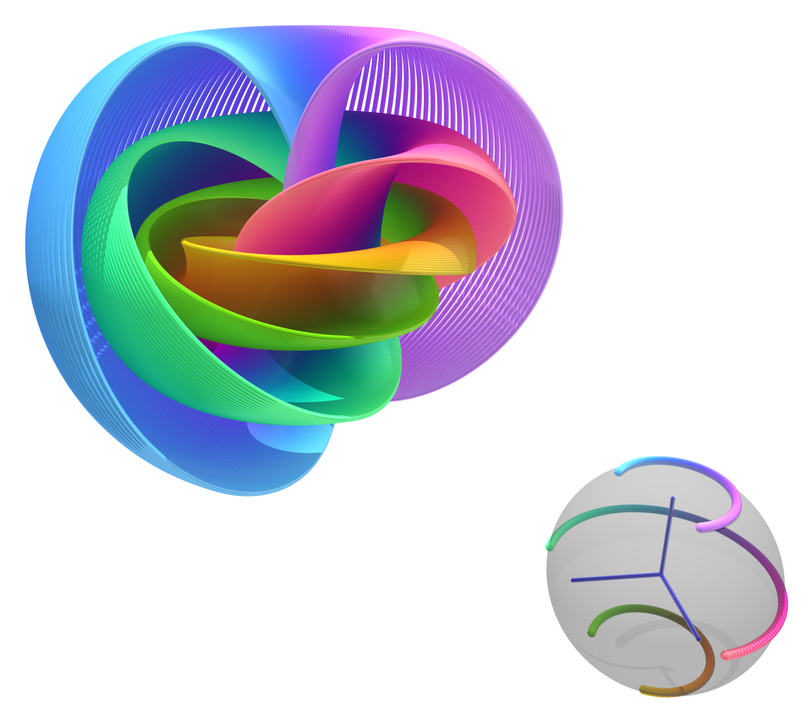
\includegraphics[width=0.5\textwidth]{hopf-fibration.png}
    \caption{The Hopf fibration. Image by Niles Johnson, CC BY-SA 3.0 \url{https://creativecommons.org/licenses/by-sa/3.0}, via Wikimedia Commons.}
    \label{hopf-fig}
\end{figure}
\subsection{Quaternionic projective space $\HP{n}$ and beyond}
The 2-dimensionality of $\mathbb{C}$ ensured that the n-cells of $\CP{n}$ were well spread in dimension, leading to an easy homology calculation. One can wonder if the same method can be applied to the higher dimensional extension of $\mathbb{R}$. Indeed we can! The quaternions $\mathbb{H}$ is a four-dimensional extension of $\mathbb{R}$. It is \textit{not} a field, as it is not commutative. However, it retains all the other requirements of a field, importantly does not have zero-divisors. Rings where every nonzero element has a multiplicative inverse are called \defn{division algebras}. The fact that $\mathbb{H}$ is a division algebra is what allows us to use the same argument as before on the Quaternionic projective space $\HP{n}$.

\begin{prop}
$\HP{n}$ has a cell structure with a $4k$-cell for $0\leq k\leq n$. As a consequence, $$H_k(\HP{n})=\begin{cases}\mathbb{Z} & k=0\text{ mod } 4 , 0\leq k\leq 4n \\ 0 & \text{otherwise}\end{cases}$$
\end{prop}

\begin{proof}
As in previous cases, $\HP{0}=\bullet$, as $z\sim 1$ for every $z\in \mathbb{H}$ by division by $z$. For general $\HP{n}$ we will proceed by induction. $\HP{n}=\mathbb{H}^{n+1}/\sim$
$$(z_1,\dots,z_{n+1})\sim h(z_1,\dots,z_{n+1}), \forall h\in \mathbb{H}$$
If $z_{n+1}\neq 0$, we can divide by $z_{n+1}$ to find a set of unique representations
$$\{(u_1,\dots,u_n,1)\}\homeo \mathbb{H}^n\homeo int(D^{4n})$$
The boundary of this set in $\HP{n}$ is the quotient 
$$\{(z_1,\dots,z_n,0)\}/\sim \homeo \HP{n-1}$$
We can therefore give $\HP{n}$ the CW-structure of $\HP{n-1}$, with an additional $4n$-cell, mapped onto $\HP{n-1}$ via the projection on its boundary $p:S^{4n-1}\rightarrow \HP{n-1}$. By induction, $\HP{n}$ has the CW-structure stated in the proposition. Since $\HP{n}$ has no $m$-cells in adjacent dimensions, its $m$-th homology group is the free abelian group generated by its $m$-cell (or lack thereof).
\end{proof}

\begin{remark}
Notice that $\HP{1}$ has a 0-cell and a 4-cell, and is therefore homeomorphic to $S^{4}$. As in Remark \ref{hopf}, the gluing map of the 8-cell of $\HP{2}$ onto $\HP{1}\iso S^{4}$, therefore gives a "Hopf"-map $S^7\rightarrow S^4$ with the property that the preimage of a point is a "great" copy of $S^3$. If there was a way to keep extending $\mathbb{R}$ to a division algebra for every positive power of two we could repeat this process, yielding "Hopf"-maps from $S^{2^n-1}$ to $S^{n-1}$ for all $n>0$. However, this is false!!! The non-existence of such maps for $n>4$ proves there are no $2^n$-dimensional division algebras of $\mathbb{R}$ for $n>4$.
\end{remark}
\section{Homology of $\S{n}$}


\section{Appendix}
\renewcommand\thesubsection{\Alph{subsection}}

\subsection{Proof of the Braid Lemma}
In this section, we give the rest of the proof of Lemma \ref{braid-lemma}.

\begin{proof}
Recall the following commutative braid lemma diagram, where we have assumed the sequence indexed by $f_i$ is a chain complex, and the other sequences are exact sequences. 

% https://tikzcd.yichuanshen.de/#N4Igdg9gJgpgziAXAbVABwnAlgFyxMJZARgBpiBdUkANwEMAbAVxiRAEEQBfU9TXfIRRkAzFVqMWbAELdeIDNjwEiAVnLj6zVohABxOXyWC1pMdS1TdACUML+yocgBMpZ5sk6QAYTuKBKigiGhaebAAifg4mQWYe2mwAolHGgcgALG7xViAAYikBTgBsWaEJugCSBY5EAAyktdle1THI9e5lOQDyLWn16U1svU4A7HGdXgDSw0RjlBNsAFLc4jBQAObwRKAAZgBOEAC2SPUgOBBImRLlIDsA+sR2+0eX1OdIJdc5985PB8eIT7vRDBEAAIxgYCgSAAtOkAJwLXT3ER-F6IMhnC6IK6WLwACweaIBV2B6i+BLuvx4u3+SHJwNc4Mh0JxiIpbEJqJptzpiFOZOoEKhl3ZeLY6yJPOeAMxwM+wtZcLFYV0ACspfIZR83tixhz1VTiUh9YykSANdytXyGXrzZLqdb0absaDxbpJVbaejQcCABzm+7pY2IJn+82E4PSvns4GnRVIES1aPo4gC7Gnd0gSW1ENp3VITFZjW5lOyuXYzEJxAwpNlpABrGFplZwmqEON4HEN2q253dv10MFjE9m4a4NClmiwe+yst3uSifMkU1hFcChcIA
\begin{tikzcd}
{} \arrow[rd, bend left]              &                                                      &                                       &                                                      &                                       &                                                      &                                       &   \\
                                      & A \arrow[rd, "f_1"] \arrow[rr, "g_1", bend left=49]  &                                       & D \arrow[rr, "h_3", bend left=49] \arrow[rd, "g_2"]  &                                       & G \arrow[rd, "h_4"] \arrow[rr, "j_4", bend left=49]  &                                       & J \\
O \arrow[ru, "g_0"] \arrow[rd, "j_0"] &                                                      & C \arrow[rd, "f_2"] \arrow[ru, "h_2"] &                                                      & F \arrow[ru, "j_3"] \arrow[rd, "g_3"] &                                                      & I \arrow[rd, "h_5"] \arrow[ru, "f_5"] &   \\
                                      & B \arrow[ru, "h_1"] \arrow[rr, "j_1", bend right=49] &                                       & E \arrow[rr, "f_3", bend right=49] \arrow[ru, "j_2"] &                                       & H \arrow[ru, "f_4"] \arrow[rr, "g_4", bend right=49] &                                       & K \\
{} \arrow[ru, bend right]             &                                                      &                                       &                                                      &                                       &                                                      &                                       &  
\end{tikzcd}

We have shown that $ker(f_2)\subseteq im(f_1)$ and need to show that $ker(f_3)\subseteq im(f_1)$ and $ker(f_4)\subseteq im(f_3)$.

\begin{enumerate}[(a)]
\item $ker(f_3)\subseteq im(f_1)$.

Let $x\in E$ be s.t. $f_3(x)=0$. By commutativity, $g_3j_2(x)=0$, so $j_2(x)\in ker(g_3)=im(g_2)$. Then $\exists x_1\in D$ s.t. $g_2(x_1)=j_2(x)$. It satisfies $h_3(x_1)=j_3g_2(x_1)=j_3j_2(x)=0$, as $(j_i)$ is a chain complex. So $x_1\in ker(h_3)=im(h_2)$. Therefore there exists $x_2\in C$ s.t. $h_2(x_2)=x_1$. This element is such that $j_2f_2(x_2)=g_2h_2(x_2)=g_2(x_1)=j_2(x)$. We therefore have $j_2(f_2(x_2)-x)=0$.

Let $x_3:=f_2(x_2)-x$. Then $x_3\in ker(j_2)=im(j_1)$. Let $x_4\in B$ be s.t. $j_1(x_4)=x_3$. $x_4$ is such that $f_2h_1(x_4)=j_1(x_4)=x_3=f_2(x_2)-x$.
Finally, we see that $x=f_2(x_2-h_1(x_4)),$ so $x\in im(f_2)$ as required.

\item $ker(f_4\subseteq im(f_3)$. 

Let $x\in H$ be s.t. $f_4(x)=0$. Then $0=h_5f_4(x)=g_4(x)$. So $x\in ker(g_4)=im(g_3)$. Let $x_1\in F$ be s.t. $g_3(x_1)=x$. Then $h_4j_3(x_1)=f_4g_3(x_1)=f_4(x)=0$
So $j_3(x_1)\in ker(h_4)=im(h_3)$. Let $x_2\in D$ be s.t. $h_3(x_2)=j_3(x_1)$. Then $j_3(x_1)=j_2g_2(x_2)$, s.t. $x_3:=g_2(x_2)-x_1\in \ker(j_3)=im(j_2)$. Let $x_4\in E$ be s.t. $j_2(x_4)=x_3$. Then $f_3(x_4)=g_3j_2(x_4)=g_3(x_3)=g_3(g_2(x_2)-x_1)=-g_3(x_1)=-x$. Therefore $x=f_3(-x_4)$, and $x\in im(f_3)$ as required.
\end{enumerate}\end{proof}
\newpage\bibliography{bibtex}
\end{document}
